\documentclass[12pt]{article}
\usepackage[a4paper, inner=1.5cm, outer=3cm, top=2cm,bottom=3cm, bindingoffset=1cm]{geometry}
\usepackage[english]{babel}
\usepackage[utf8x]{inputenc}
\usepackage[nottoc]{tocbibind}
\usepackage{import}
\usepackage{nomencl}
\usepackage{amsmath}
\usepackage{tikz}
\usepackage[maxfloats=256]{morefloats}
\usepackage{booktabs}
\usepackage{graphicx}
\usepackage{eso-pic}
\usepackage{hyperref}
\usepackage{pdflscape}
\usepackage{adjustbox}
\graphicspath{ {./images/} }
\usepackage{capt-of} 
\usepackage{listings}
\usepackage{xcolor}
\usepackage{multirow}
\usepackage{setspace}
\definecolor{codegreen}{rgb}{0,0.6,0}
\definecolor{codegray}{rgb}{0.5,0.5,0.5}
\definecolor{codepurple}{rgb}{0.58,0,0.82}
\definecolor{backcolour}{rgb}{0.95,0.95,0.92}
%\usepackage{array}
%\renewcommand{\arraystretch}{1.5}
\maxdeadcycles=1000
 
\lstdefinestyle{mystyle}{
    backgroundcolor=\color{backcolour},   
    commentstyle=\color{codegreen},
    keywordstyle=\color{magenta},
    numberstyle=\tiny\color{codegray},
    stringstyle=\color{codepurple},
    basicstyle=\ttfamily\footnotesize,
    breakatwhitespace=false,         
    breaklines=true,                 
    captionpos=b,                    
    keepspaces=true,                 
    numbers=left,                    
    numbersep=5pt,                  
    showspaces=false,                
    showstringspaces=false,
    showtabs=false,                  
    tabsize=2
}
 
\lstset{style=mystyle}

\begin{document}
\begin{titlepage}
\newcommand{\HRule}{\rule{\linewidth}{0.5mm}} 
\center
\doublespacing
\textbf{\Huge MACHINE LEARNING FOR PREDICTING DIABETES MELLITUS}
\\
\singlespacing
\Large
\vspace{3cm}
A project report submitted in partial fulfilment of the requirement for the degree of\\
\vspace{1cm}
\textbf{Bachelor in Science\\In\\Computer Science}
\\by\\
\vspace{1cm}
\Large
Alexander Roque Rodrigues
\\
\normalsize
\vspace{0.5cm}
under the supervision of
\\
\Large
Ashweta Anand Fondekar
\\
\vspace{3cm}
\Large
\textbf{PARVATIBAI CHOWGULE COLLEGE OF ARTS \& SCIENCE AUTONOMOUS}
\\June 2019
\end{titlepage}

%declaration
\onehalfspacing
%\doublespacing
\newpage
\vspace{15cm}
\begin{center}
\Huge{\textbf{Declaration by Candidate}}\\
\normalsize
\vspace{5cm}
I declare that this project report has been prepared by me and to the best of my
knowledge, it has not previously formed the basis for the award of any diploma or degree by
any other University.\\
\vspace{5cm}
Alexander Roque Rodrigues\\

Student
\end{center}
\newpage
\vspace{15cm}

\begin{center}
\Huge{\textbf{Certificate by Supervisor}}\\
\normalsize
\vspace{5cm}
Certified that the Project Report is a record of work done by the candidate himself/herself/themselves under my guidance during the period of study and that to the best of my knowledge, it has not previously formed the basis of the award of any degree or diploma of any other University.\\
\vspace{5cm}
Ashweta Anand Fondekar\\

Project Supervisor
\end{center}

\clearpage
\newpage
\section{Consolidated Marksheet of Project Work}
Name of the department: Computer Science\\
Name of the examination:\\
Year:\\
\begingroup
\setlength{\tabcolsep}{10pt} % Default value: 6pt
\renewcommand{\arraystretch}{1.5} % Default value: 1
\begin{table}[ht]
\begin{tabular}{|c|c|c|c|c|c|}
\hline
\multirow{2}{*}{Roll Number} & \multirow{2}{*}{Name of Candidate}         & \multicolumn{2}{c|}{\begin{tabular}[c]{@{}c@{}}Marks\\ awarded\\ by Internal\\ Examiner\\ (/50)\end{tabular}}     & \begin{tabular}[c]{@{}c@{}}Marks\\ awarded\\ by External\\ Examiner\\ (/50)\end{tabular} & \begin{tabular}[c]{@{}c@{}}Total\\ Marks\\ awarded\\ (/100)\end{tabular} \\ \cline{3-6} 
                             &                                            & \begin{tabular}[c]{@{}c@{}}Sem 5\\ (/15)\end{tabular} & \begin{tabular}[c]{@{}c@{}}Sem 6\\ (/35)\end{tabular} & \multirow{3}{*}{}                                                                    & \multirow{3}{*}{}                                                        \\ \cline{1-4}
SU170331                     & \multirow{2}{*}{Alexander Roque Rodrigues} & \multirow{2}{*}{}                                     & \multirow{2}{*}{}                                     &                                                                                      &                                                                          \\ \cline{1-1}
\multicolumn{1}{|l|}{}       &                                            &                                                       &                                                       &                                                                                      &                                                                          \\ \hline
\end{tabular}
\end{table}
\endgroup
\vspace{4cm}
\begin{flushleft}
External Examiner/ Faculty Council\\
Place:\\
Date:\\
\end{flushleft}


\begin{flushright}\vspace{-2cm} Internal Examiner\end{flushright}

\vspace{5cm}
\begin{flushleft}
Checked and Countersigned\\
College Seal
\end{flushleft}



\clearpage
\newpage
\section{Acknowledgements}
First of all, I am thankful to God as without Him by my side, I would not be here;
for the strength given to me to fight against all adversities. The following document
summarizes a year’s worth of effort, frustration and achievement. There are several
people with whom I am thankful for their contribution in this work.

I am highly indebted to Tr. Ashweta Anand Fondekar for her guidance and constant supervision as well as for providing necessary information regarding the project and also for their support in completing the project. I would also like to express my gratitude towards my parents for their kind co-operation and encouragement which help me in completion of this project. I would also like to express my special gratitude and thanks to Sir. Kumaresh for giving me such attention and time for all the hardware related matters. My thanks and appreciations also go to my college faculty for aiding me in developing the project and people who have willingly helped me out with their abilities whenever necessary.


\newpage
\tableofcontents
\newpage
\listoffigures
\newpage
\listoftables
\newpage


\begin{abstract}
Diabetes Mellitus is a disease that prevents the body from properly expanding the
energy stored from the food consumed. The purpose of this project was to select
machine learning algorithms that are able to predict or classify a person as diabetic
or healthy based on the legacy data. The algorithms compared were KNN
Classifier, Logistic Regression, Decision Tree Classifier, Random Forest
Classifier, Gradient Boosting Classifier, Support Vector Classifier and the
Multi-Layered Perceptron. From all the above the Multi-Layered Perceptron gave
an accuracy of prediction on the dataset as ~79.70\%. To improve the performance
of the classifier, I have considered new features deduced from the currently
existing feature set a re-trained the classifier on the new dataset that I generated,
which is now able to classify the subject as diabetic or healthy with a new accuracy
of ~85.42\%. After selection of the algorithm I further advanced the platform of cluster computing to
deploy the algorithm onto and generate predictions in without any human
interference​ and also made the data available
to the users via an easy to use web application which gives them access to the
observations then stored in the database after being predicted by the algorithm
deployed on the nodes. Also an application programming interface provided additional connection facilities to interface the database with.
\end{abstract}


\section{Introduction}
In recent days, there has been a sharp increase in the cases of diabetes mellitus. Diabetes mellitus is on the rise amongst many people and the rate of contracting this lifestyle disease could be reduced significantly if proper measures and precautions were to be instilled amongst people the number of people can be reduced.

Machine learning is a growing field in computer science. With the development and introduction of many algorithms the prediction and accuracy of the predictions itself has improved substantially. Machine learning and healthcare systems are also becoming increasingly popular in the healthcare sector.

Machine learning is also becoming a great contender to traditional algorithms. Modern Machine Learning Algorithms are able to overcome strictly static program instructions and make data-driven predictions that help companies make decisions with minimal human intervention. IDC forecasts that spending on Machine Learning will grow from \$12 billion in 2017 to \$57.6 billion by 2021 \cite{dzone}. Cluster Computing or High-Performance computing frameworks is a form of computing in which bunch of computers (often called nodes) that are connected through a LAN (local area network) so that, they behave like a single machine. A computer cluster help to solve complex operations more efficiently with much faster processing speed, better data integrity than a single computer and they are mostly used for critical applications. These are now capable of housing machine learning algorithms.

The project encompasses the qualities of Remote Patient Monitoring (RPM)\cite{rpm} and Clinical Decision Support (CDS)\cite{cds}. RPM provides medical facilities that have the ability to transmit patient data to healthcare professionals who might very well be halfway around the world. RPM can monitor blood glucose levels and blood pressure. It is particularly helpful for patients with chronic conditions such as type 2 diabetes, hypertension, or cardiac disease. Data collected and transmitted via PRM can be used by a healthcare professional or a healthcare team to detect medical events such as stroke or heart attack that require immediate and aggressive medical intervention. Data collected may be used as part of a research project or health study. RPM is a life-saving system for patients in remote areas who cannot access face-to-face health care. CDS analyzes data from clinical and administrative systems. The aim is to assist healthcare providers in making informed clinical decisions. Data available can provide information to medical professions who are preparing diagnoses or predicting medical conditions like drug interactions and reactions. CDS tools filter information to assist healthcare professionals in caring for individual clients. 

To extend the functionality of the system I have coded an algorithm that distributes the workloads across nodes in a distributed computing environment, built a website that displays the readings of the subject measured by a doctor and lastly a simple API written in node js that can interface with our database to provide scalability. All the software coded here has been coded using a VCS (Version Control System) namely GitHub to track versions of software and make bug tracking and patching of software easy. Updates across all computers are also easily achieved using a VCS.

\subsection{Document Structure}
The document is organized as follows:
\begin{itemize}
\item \texttt{Introduction:} this section aims to introduce the project to the reader.
\item \texttt{Objective:} the objective of the document defines the difference between existing technology and equipment and the end result that the project hopes to acheive.
\item \texttt{Project Rationale:} this section is for understanding the need for the application and research of the project in the real world.
\item \texttt{Review of Literature:} the section containing review of literature sheds light on the previous experiments and researches carried out by esteemed researchers and scientist prior to us.
\item \texttt{Hardware Requirements:} This section contains the hardware requirements to build the distributed computing environment and the other networking components that are used in the process.
\item \texttt{Technology Stack:} this part deals with the frameworks and softwares used to realise the project objective.
\item \texttt{Methods and Material:} this section encompasses the methods and techniques resorted to derive results and the data sources used in the process.
\item \texttt{Results:} this section contains the final results of all the investigative work carried out.
\item \texttt{Algorithm for Load Distribution:} The working behind the load balancing algorithm written in Python.
\item \texttt{The Web User Interface:} this section specifies the functionalities of the software and lays down instruction of use for the doctor and the patient.
\item \texttt{The Application Programming Interface:} Application programming interfaces are important tools and this section elaborates on the use and how to use the API with the database.
\item \texttt{Final Conclusion and Future Work:} this final chapter, gives a review of the work and make a reflection about the achievements accomplished. Some ideas to improve the current work are also given in the last section.
\item \texttt{Tables:} this section contains tables generated during the exploratory data analysis phase and the profiling and benchmarking stages of the project.
\item \texttt{Function Syntax:} this section contains the syntax reference with a list of parameters available for the libraries.
\item \texttt{Exploratory Data Analysis Images:} this section is a section to present all the findings in the form of visuals to the reader to understand and follow the study carried out on the data.
\item \texttt{Web and API Interface Images:} a section containing the screenshots of the web user interface and the working model of the API created to access the database with.
\end{itemize}


\clearpage
\newpage
\section{Objective}
\subsection{Existing System}
Currently, there exist only systems for monitoring diabetes. Examples of these begin Medtronic\cite{medtronic} and Onetouch\cite{onetouch} are used for instantaneous results. There are also multitudes of researches being carried out on diabetic patient and looking for newer traits that can help predict the onset of the sickness.

\subsection{Proposed System}
The objective of this project is to select an algorithm that is capable of classifying a healthy person from a diabetic person. After which the selected algorithm will be deployed to a group of computers which will help us expand the computing capabilities further than a single computer. The model should then write to a database than can be queried to present data to the users who will interface the said program. The software should also be extensible and scalable in nature to accomodate load in terms of processing power and capable of being interface with other applications and products to expand domain use.

\newpage
\section{Project Rationale}

Diabetes is a chronic disease that occurs either when the pancreas does not produce enough insulin or when the body cannot effectively use the insulin it produces. Insulin is a hormone that regulates blood sugar. Hyperglycemia, or raised blood sugar, is a common effect of uncontrolled diabetes and over time leads to serious damage to many of the body's systems, especially the nerves and blood vessels.

Taking a look at the number of people with diabetes, the count has risen from 108 million in 1980 to 422 million in 2014.
The global prevalence of diabetes among adults over 18 years of age has risen from 4.7\% in 1980 to 8.5\% in 2014. Diabetes prevalence has been rising more rapidly in middle-income and low-income countries.
Diabetes as a disease is a major cause of blindness, kidney failure, heart attacks, stroke and lower limb amputation amongst those who recognise the fatal disease late in life.
In 2016, an estimated 1.6 million deaths were directly caused by diabetes. Another 2.2 million deaths were attributable to high blood glucose in 2012. Almost half of all deaths attributable to high blood glucose occur before the age of 70 years. WHO estimates that diabetes was the seventh leading cause of death in 2016. A healthy diet, regular physical activity, maintaining a normal body weight and avoiding tobacco use are ways to prevent or delay the onset of type 2 diabetes. Diabetes can be treated and its consequences avoided or delayed with diet, physical activity, medication and regular screening and treatment for complications. In 2014, 8.5\% of adults aged 18 years and older had diabetes. In 2016, diabetes was the direct cause of 1.6 million deaths and in 2012 high blood glucose was the cause of another 2.2 million deaths.

Diabetes patients are segregated into types. Type 1 diabetes is characterized by deficient insulin production and requires daily administration of insulin. The cause of type 1 diabetes is not known and it is not preventable with current knowledge. A person with type 1 diabetes may have symptoms like excessive excretion of urine, thirst, constant hunger, weight loss, vision changes, and fatigue. These symptoms may occur suddenly.

Type 2 diabetes results from the body’s ineffective use of insulin. Type 2 diabetes comprises the majority of people with diabetes around the world, and is largely the result of excess body weight and physical inactivity. Symptoms may be similar to those of type 1 diabetes, but are often less marked. As a result, the disease may be diagnosed several years after onset, once complications have already arisen.

Until recently, this type of diabetes was seen only in adults but it is now also occurring increasingly frequently in children.

Gestational diabetes is another type of diabetes where hyperglycemia with blood glucose values above normal but below those diagnostic of diabetes, occurring during pregnancy. Women with gestational diabetes are at an increased risk of complications during pregnancy and at delivery. They and their children are also at increased risk of type 2 diabetes in the future. Gestational diabetes is diagnosed through prenatal screening, rather than through reported symptoms.

Untreated diabetes can damage the heart, blood vessels, eyes, kidneys, and nerves. Adults with diabetes have a two- to three-fold increased risk of heart attacks and strokes. Combined with reduced blood flow, neuropathy (nerve damage) in the feet increases the chance of foot ulcers, infection and eventual need for limb amputation. Diabetic retinopathy is an important cause of blindness, and occurs as a result of long-term accumulated damage to the small blood vessels in the retina. 2.6\% of global blindness can be attributed to diabetes. Diabetes is among the leading causes of kidney failure.

Early diagnosis can be accomplished through relatively inexpensive testing of blood sugar. Treatment of diabetes involves diet and physical activity along with lowering blood glucose and the levels of other known risk factors that damage blood vessels. Tobacco use cessation is also important to avoid complications. \cite{alberti_zimmet_2004}\cite{internationaldiabetesfederation}

\newpage
\section{Review of Literature}

Examining Kumari and Chitra \cite{kumarandchitra} research, they also achieved an accuracy of 78\% with the support vector machine algorithm and the radial basis function kernel function incoorporating the PIMA 1 database obtained from the UCI Repository of Machine Learning Repository. 

W. Yu, T. Liu, R. Valdez, M. Gwinn, and M. Khoury \cite{biomedcentral} in their research used Support Vector Machines to see how accurately it can perform diagnosis of diabetes. The approach consisted in creating two classification schemes: 
\begin{enumerate}
\item Diagnosed as diabetic vs. no diabetes.
\item Undiagnosed diabetes or pre-diabetes vs. no diabetes.
\end{enumerate}
Data between 1999 and 2004 from the National Health and Nutrition Examination Survey was used in this work. Results showed that
Radial Basis Function kernel function performed better in the first classification scheme with accuracy of 83.47\% and for the second one, the linear kernel function was the best with an accuracy of 73.18\%. They also compared these values with the
ones obtained by a logistic regression analysis and concluded that there is no statistical difference in their discriminative power, i.e., the performance of both methods are equal.

Kemal Polat and Salih Güneş' research document\cite{POLAT2007702} suggested a method to attain better results in this problem. In their study, they used Principle Component Analysis to reduce the number of features present in the dataset. After that, diabetes’ diagnosis is performed by a neuro-fuzzy inference classification system. This approach reached an accuracy of 89.47\%.

In accordance with research from Kemal Polat and Salih Güneş and Ahmet Arslan\cite{POLAT2008482} compare the results obtained with Least Square Support Vector Machine and their method that is a combination of Generalized Discriminant Analysis (GDA) and LS-SVM. GDA is used as a pre-processing data method while LS-SVM classifies the data. While they got an accuracy of 78.21\% with LS-SVM, they accomplished 79.16\% with GDA-LS-SVM.

A modified version of support vector machine algorithm named Laplacian Support Vector Machine (LapSVM) was tested by Jiang Wu, Yuan-Bo Diao, Meng-Long Li, Ya-Ping Fang and Dai-Chuan Ma \cite{semisupervised}. In this study, a LapSVM was trained as a fully supervised learning classifier and another one as a semi-supervised learning classifier. The accuracy results achieved were 79.17\% and 82.29\%, respectively.

\clearpage
\newpage
\section{Hardware Requirements}
\subsection{Hardware Components}
\subsubsection{Raspberry Pi}
According to raspberrypi.org\cite{rpi}, the Raspberry Pi 3 Model B is the earliest model of the third-generation Raspberry Pi. It replaced the Raspberry Pi 2 Model B in February 2016. Some of the key features of this single board computer or SBC are:
\begin{itemize}
\item Quad Core 1.2GHz Broadcom BCM2837 64bit CPU.
\item 1GB RAM.
\item BCM43438 wireless LAN and Bluetooth Low Energy (BLE) on board.
\item 100 Base Ethernet.
\item 40-pin extended GPIO.
\item 4 USB 2 ports.
\item Full size HDMI.
\item Micro SD port for loading the operating system and storing data.
\end{itemize}
In this project I will be using 3 Raspberry Pi's to implement a cluster and deploy the machine learning algorithm on.

\subsubsection{Switch}
A network switch was used in the project to make up for the lack of ethernet ports available on the router.

\subsubsection{Router}
A router is required to assign internet protocol addresses to the nodes using dynamic host control protocol (DHCP). The router also is responsible for displaying the nodes connected to the network thereby displaying host names and making it more easier to capture the addresses of each node.

\subsubsection{Master Node}
The master node is assigned the task of managing the the slave nodes connected to the network. The master node and the slave nodes should be connected to the same database to run and execute queries. The master node shall also be assigned with the task of killing a particular process or shutting down a particular node if required.

\subsubsection{Slave Node}
The slave nodes are to be configured with the selected algorithm and are the most vital part of the structure. The slave nodes will be responsible for receiving instructions from the master node and will be responsible for learning from the dataset and then can generate predicted outcomes for the patient records received from the master. 

\subsubsection{Database}
The database will store all the records for the patients and doctors. The database is a SQL database that will not be subjected to a change in the database schema structure for consistency.

\subsubsection{Web Server}
Since it would be a waste if the data was generated and merely stored in the database, the web server provides a simplified interface for the doctor and the patients to read the data from the database.

\clearpage
\newpage
\subsection{Functionality Specifications}
The main function of this project is to enable the doctors to advise their patients with the help of the prediction software. The system should be accessible to the patient as well as the doctor, therefore it should have a web interface for the two parties to interact with.

\subsubsection{Functionalities for Master Nodes}
As the master nodes:
\begin{itemize}
\item Control chunk size.
\item Remotely update the slave nodes.
\item Check the status of nodes.
\item Control the SQL database.
\end{itemize}

\subsubsection{Functionalities for Slave Nodes}
\begin{itemize}
\item Should have the machine learning algorithm tuned as per specifications.
\item Remote update should be possible.
\item Remote connectivity should be possible
\end{itemize}


\clearpage
\newpage
\section{Technology Stack}
\subsection{Python}
\subsubsection{Pandas}
Pandas, is a library that is required for loading the comma separated value file into python. Pandas is a package for data manipulation and analysis. In particular, it offers data structures and operations for manipulating numerical tables and time series.\cite{pandas}

\subsubsection{Sklearn}
Scikit-learn is a free software machine learning library for the Python programming language. It features various classification, regression and clustering algorithms including support vector machines, random forests, gradient boosting, k-means and DBSCAN, and is designed to inter-operate with the Python numerical and scientific libraries NumPy and SciPy.\cite{scikit}

\subsubsection{Numpy}
NumPy is a library for the Python programming language, adding support for large, multi-dimensional arrays and matrices, along with a large collection of high-level mathematical functions to operate on these arrays. NumPy is open-source software and has many contributors.\cite{numpy}

\subsubsection{Itertools}
The itertools module standardizes a core set of fast, memory efficient tools that are useful by themselves or in combination. Together, they form an “iterator algebra” making it possible to construct specialized tools succinctly and efficiently in pure Python.\cite{itertools}

\subsection{MYSQL}
MySQL is an open-source relational database management system. MySQL is free and open-source software under the terms of the GNU General Public License, and is also available under a variety of proprietary licenses. MySQL was owned and sponsored by the Swedish company MySQL AB, which was bought by Sun Microsystems (now Oracle Corporation). MySQL is a component of the LAMP web application software stack (and others), which is an acronym for Linux, Apache, MySQL, Perl/PHP/Python. MySQL is used by many database-driven web applications, including Drupal, Joomla, phpBB, and WordPress. MySQL is also used by many popular websites, including Facebook, Flickr, MediaWiki, Twitter and YouTube.\cite{mysql}

\subsection{Apache Web Server}
The Apache HTTP Server, colloquially called Apache, is free and open-source cross-platform web server software, released under the terms of Apache License 2.0. Apache is developed and maintained by an open community of developers under the auspices of the Apache Software Foundation. The vast majority of Apache HTTP Server instances run on a Linux distribution, but current versions also run on Microsoft Windows and a wide variety of Unix-like systems. Past versions also ran on OpenVMS, NetWare, OS/2 and other operating systems, including ports to mainframes.\cite{apache}

\subsection{PHP}
PHP is a general-purpose programming language originally designed for web development. PHP originally stood for Personal Home Page,
but it now stands for the recursive initialism PHP: Hypertext Preprocessor. PHP code may be executed with a command line interface (CLI), embedded into HTML code, or used in combination with various web template systems, web content management systems, and web frameworks. PHP code is usually processed by a PHP interpreter implemented as a module in a web server or as a Common Gateway Interface (CGI) executable. The web server outputs the results of the interpreted and executed PHP code, which may be any type of data, such as generated HTML code or binary image data. PHP can be used for many programming tasks outside of the web context, such as standalone graphical applications and robotic drone control.\cite{php}

\subsection{AJAX}
Ajax is a set of web development techniques using many web technologies on the client side to create asynchronous web applications. With Ajax, web applications can send and retrieve data from a server asynchronously (in the background) without interfering with the display and behavior of the existing page. By decoupling the data interchange layer from the presentation layer, Ajax allows web pages and, by extension, web applications, to change content dynamically without the need to reload the entire page.\cite{ajax}

Ajax is not a single technology, but rather a group of technologies. HTML and CSS can be used in combination to mark up and style information. The webpage can then be modified by JavaScript to dynamically display—and allow the user to interact with—the new information. The built-in XMLHttpRequest object, or since 2017 the new "fetch()" function within JavaScript, is commonly used to execute Ajax on web pages allowing websites to load content onto the screen without refreshing the page. Ajax is not a new technology, or different language, just existing technologies used in new ways.

\subsection{GitHub}
GitHub is a global company that provides hosting for software development version control using Git. It offers all of the distributed version control and source code management (SCM) functionality of Git as well as adding its own features. It provides access control and several collaboration features such as bug tracking, feature requests, task management, and wikis for every project.\cite{git}

\subsection{SSH}
Secure Shell is a cryptography network protocol for operating network services securely over an unsecured network. Typical applications include remote command-line, login, and remote command execution, but any network service can be secured with SSH. The SSH is used to communicate between the master and slave nodes.\cite{ssh}

\subsection{Node.js}
Node.js is an open-source and cross-platform JavaScript reunite environment. Node.js runs the V8 JavaScript engine, the core of Google Chrome, outside of the browser. This allows Node.js to be very performant.

A Node.js app is run in a single process, without creating a new thread for every request. Node.js provides a set of asynchronous I/O primitives in its standard library that prevent JavaScript code from blocking and generally, libraries in Node.js are written using non-blocking paradigms, making blocking behavior the exception rather than the norm.

When Node.js needs to perform an I/O operation, like reading from the network, accessing a database or the file-system, instead of blocking the thread and wasting CPU cycles waiting, Node.js will resume the operations when the response comes back.

This allows Node.js to handle thousands of concurrent connections with a single server without introducing the burden of managing thread concurrency, which could be a significant source of bugs.

Node.js has a unique advantage because millions of front-end developers that write JavaScript for the browser are now able to write the server-side code in addition to the client-side code without the need to learn a completely different language.

In Node.js the new ECMAScript standards can be used without problems, as there is no waiting time for all users to update their browsers. Developers are in charge of deciding which ECMAScript version to use by changing the Node.js version, and you can also enable specific experimental features by running Node.js with flags.\cite{nodejs}

\subsubsection{Express.js}
Express.js, or simply Express, is a web application framework for Node.js, released as free and open-source software under the MIT License. It is designed for building web applications and APIs. It has been called the de facto standard server framework for Node.js.\cite{expressjs}

\subsubsection{Body Parser}
Being able to parse a payload given to a node.js back end typically via a post request is a very common task when doing something with express.js. As such there is a built in way to quickly do this thanks to the body-parser module that is included with every express.js install.\cite{bodyparser}

\clearpage
\newpage
\section{Methods and Material}
\vspace{5cm}
\begin{figure}[h]
\centering

\tikzset{every picture/.style={line width=0.75pt}} %set default line width to 0.75pt        

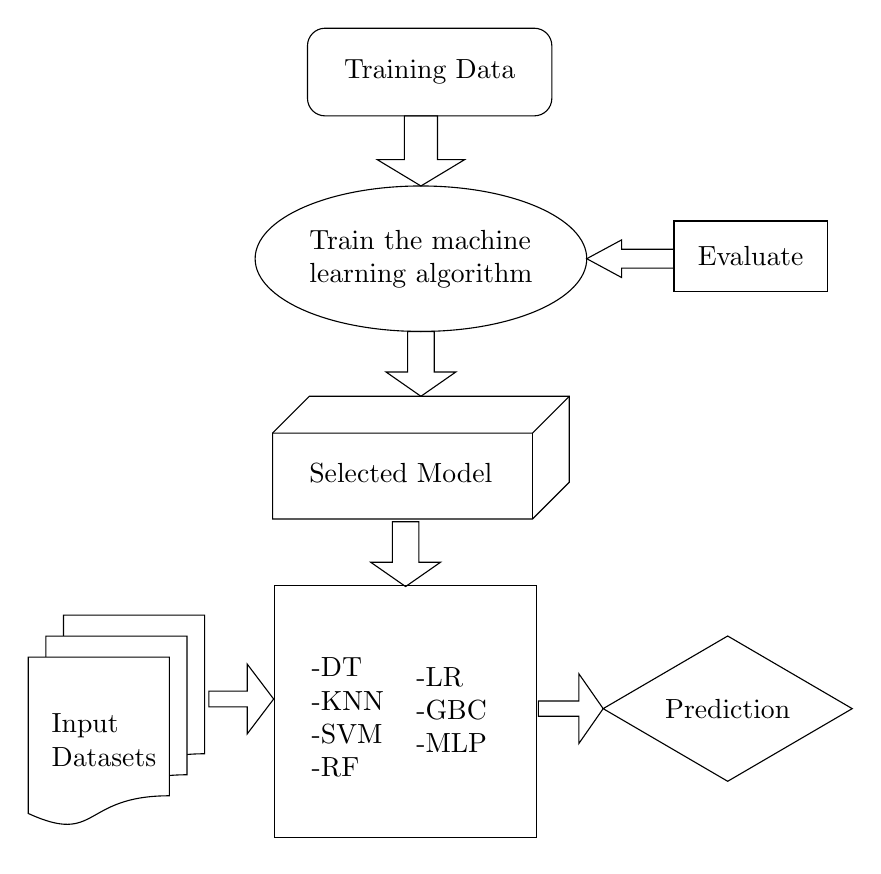
\begin{tikzpicture}[x=0.75pt,y=0.75pt,yscale=-1,xscale=1]
%uncomment if require: \path (0,466); %set diagram left start at 0, and has height of 466

%Rounded Rect [id:dp6337385239032856] 
\draw   (259.55,38.44) .. controls (259.55,33.78) and (263.33,30) .. (267.99,30) -- (368.83,30) .. controls (373.49,30) and (377.27,33.78) .. (377.27,38.44) -- (377.27,63.78) .. controls (377.27,68.44) and (373.49,72.22) .. (368.83,72.22) -- (267.99,72.22) .. controls (263.33,72.22) and (259.55,68.44) .. (259.55,63.78) -- cycle ;
%Down Arrow [id:dp3985906249685618] 
\draw   (293.18,93.33) -- (306.22,93.33) -- (306.22,72.22) -- (322.19,72.22) -- (322.19,93.33) -- (335.23,93.33) -- (314.2,106) -- cycle ;
%Shape: Ellipse [id:dp30062854070983147] 
\draw   (234.32,141.04) .. controls (234.32,121.69) and (270.08,106) .. (314.2,106) .. controls (358.32,106) and (394.09,121.69) .. (394.09,141.04) .. controls (394.09,160.4) and (358.32,176.09) .. (314.2,176.09) .. controls (270.08,176.09) and (234.32,160.4) .. (234.32,141.04) -- cycle ;
%Right Arrow [id:dp11710564652522826] 
\draw   (436.14,145.58) -- (410.91,145.58) -- (410.91,150.12) -- (394.09,141.04) -- (410.91,131.97) -- (410.91,136.51) -- (436.14,136.51) -- cycle ;
%Shape: Rectangle [id:dp19028837916577346] 
\draw   (436.14,122.89) -- (510,122.89) -- (510,156.67) -- (436.14,156.67) -- cycle ;
%Shape: Cube [id:dp5027072537432922] 
\draw   (242.73,225.07) -- (260.46,207.33) -- (385.68,207.33) -- (385.68,248.71) -- (367.95,266.44) -- (242.73,266.44) -- cycle ; \draw   (385.68,207.33) -- (367.95,225.07) -- (242.73,225.07) ; \draw   (367.95,225.07) -- (367.95,266.44) ;
%Down Arrow [id:dp22764550188777388] 
\draw   (297.39,195.62) -- (307.81,195.62) -- (307.81,176.09) -- (320.6,176.09) -- (320.6,195.62) -- (331.02,195.62) -- (314.2,207.33) -- cycle ;
%Flowchart: Multidocument [id:dp8891219796914933] 
\draw  [fill={rgb, 255:red, 255; green, 255; blue, 255 }  ,fill opacity=1 ] (142,312.75) -- (210,312.75) -- (210,379.56) .. controls (167.5,379.56) and (176,403.65) .. (142,388.06) -- cycle ; \draw  [fill={rgb, 255:red, 255; green, 255; blue, 255 }  ,fill opacity=1 ] (133.5,322.87) -- (201.5,322.87) -- (201.5,389.68) .. controls (159,389.68) and (167.5,413.77) .. (133.5,398.18) -- cycle ; \draw  [fill={rgb, 255:red, 255; green, 255; blue, 255 }  ,fill opacity=1 ] (125,332.99) -- (193,332.99) -- (193,399.8) .. controls (150.5,399.8) and (159,423.89) .. (125,408.31) -- cycle ;
%Shape: Rectangle [id:dp964493388000915] 
\draw   (243.86,298.4) -- (370,298.4) -- (370,420) -- (243.86,420) -- cycle ;
%Down Arrow [id:dp34313084687696693] 
\draw   (290,287.28) -- (300.43,287.28) -- (300.43,267.76) -- (313.21,267.76) -- (313.21,287.28) -- (323.64,287.28) -- (306.82,299) -- cycle ;
%Down Arrow [id:dp14788058560327122] 
\draw   (230.5,370) -- (230.5,357) -- (212,357) -- (212,349.36) -- (230.5,349.36) -- (230.5,336.36) -- (243.24,353.18) -- cycle ;
%Down Arrow [id:dp0526621585505318] 
\draw   (390.28,374.64) -- (390.28,361.5) -- (370.76,361.5) -- (370.76,354.14) -- (390.28,354.14) -- (390.28,341) -- (402,357.82) -- cycle ;
%Shape: Diamond [id:dp4139142007908323] 
\draw   (462,322.82) -- (522,357.82) -- (462,392.82) -- (402,357.82) -- cycle ;

% Text Node
\draw (318.41,51.11) node   [align=left] {Training Data};
% Text Node
\draw (314.2,141.04) node   [align=left] {Train the machine \\learning algorithm};
% Text Node
\draw (473.07,139.78) node   [align=left] {Evaluate};
% Text Node
\draw (304.53,244.07) node   [align=left] {Selected Model};
% Text Node
\draw (161.5,373) node   [align=left] {Input\\Datasets};
% Text Node
\draw (279,362) node   [align=left] {\mbox{-}DT\\\mbox{-}KNN\\\mbox{-}SVM\\\mbox{-}RF};
% Text Node
\draw (329,358.5) node   [align=left] {\mbox{-}LR\\\mbox{-}GBC\\\mbox{-}MLP};
% Text Node
\draw (462,357.82) node   [align=left] {Prediction};


\end{tikzpicture}
\caption{\label{fig:59}Model that forms the basis of selecting machine learning algorithms.}
\end{figure}
\clearpage
\newpage

\subsection{Data Collection}
The dataset used for this project is from the UCI Machine learning repository and can be found at their respective website\cite{johannes1988using}\cite{nr}. This dataset is originally from the National Institute of Diabetes and Digestive and Kidney Diseases. The objective is to predict based on diagnostic measurements whether a patient has diabetes. Table \ref{table:2} is an outcome of the accuracy of the algorithms subjected to train and \ref{table:3} is the accuracy obtained from the tested outcomes for given sets of patients.

\subsection{Exploratory Data Analysis}
Firstly, on examining the amount of people that were recorded by the dataset, we can see that the dataset contains a total of 768 observations. We can see that 268 people are healthy, while the rest of the 500 subjects are diabetic. If put in terms of percentage, 65.1\% of the subjects are healthy and 34.9\% of subjects are diabetic.

To proceed with the exploratory data analysis, we can examine the missing values in the dataset. We can see that the dataset has multiple missing values across the columns of the dataset and furthermore, plotting of box-plots reveals that the dataset has multiple outliers. To replace these missing values with values to make the predictions more accurate we need to understand the relation of the data to the target variable. To get an understanding we can use the table \ref{table:6} for clarity on the correlation of values.

To fill the missing values in the dataset we have to consider each of the attributes. For example in the insulin parameter, I have observed that the median value for diabetic people is 169.50 muU/ml, while for the section of healthy participants the median insulin value is recorded at 102.50 muU/ml. Likewise, I carried out the observations on the other attributes of the dataset to fill the missing values via the median of healthy subjects for the healthy subjects whose insulin record is missing and diabetic insulin median for the subjects that are diabetic and do not have values in the columns.

In order to generate new values for the dataset to render more accurate outcomes we look at scatter-plots for our attributes. An example would be the Glucose vs Age scatter-plot. According to the scatter plot of glucose to age we can see that higher glucose value with increase in age, depicts the glucose level of a diabetic person.

To generate new features to improve the accuracy of classification, we have introduced new attributes into the dataset. These new attributes aim to reduce the error in prediction by making further distinctions between the diabetic subjects and the healthy subjects. The attributes \texttt{N0} to \texttt{N14} are all the subjects who are healthy from all the attributes. Since the healthy subjects are now segregated the subjects who are diabetic will now be easier to identify. This concept is      proven by looking at figure \ref{fig:49} which shows that the data in the \texttt{N} columns are more correlated since they \textbf{comprise of a majority of healthy subjects}.

The new attributes generated are given as follows:

\begin{enumerate}

\item \texttt{N0}: Body Mass Index * Skin Thickness
\item \texttt{N1}: All subjects with Age $<$ 30 and Glucose Level $<$=120
\item \texttt{N2}: All subjects with BMI $<$=30
\item \texttt{N3}: All subjects with Age $<$= 30 and Pregnancies $<$= 6
\item \texttt{N4}: All subjects with Glucose $<$= 105 and BloodPressure $<$= 80
\item \texttt{N5}: All subjects with SkinThickness $<$= 20
\item \texttt{N6}: All subjects with BMI $<$ 30 and SkinThickness $<$= 20
\item \texttt{N7}: All subjects with Glucose $<$= 105 and BMI $<$= 30
\item \texttt{N8}: Number of Pregnancies / Age of Subject
\item \texttt{N9}: All subjects with Insulin $<$ 200
\item \texttt{N10}: All subjects with Blood Pressure $<$ 80
\item \texttt{N11}: All subjects with Pregnancies $>$ 0 and $<$ 4
\item \texttt{N12}: Age of Subject * Diabetes Pedigree Function
\item \texttt{N13}: Glucose * Diabetes Pedigree Function
\item \texttt{N14}: Age * Insulin

\end{enumerate} 

{
\clearpage
\begin{landscape}
\begin{figure}[ht]
\centering
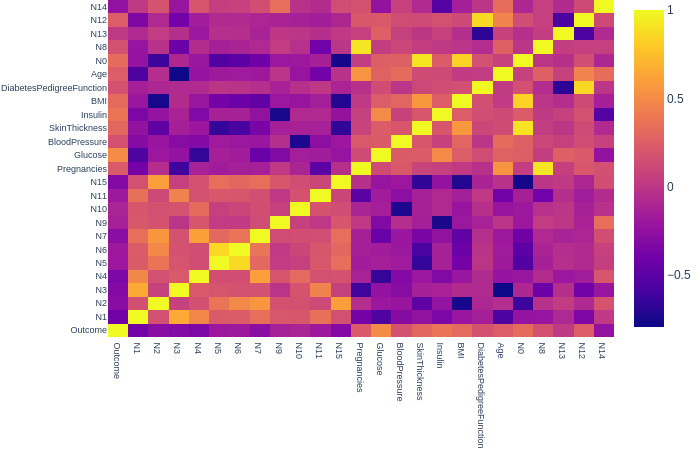
\includegraphics[width=1.5\textwidth]{newplot(42).png}
\caption{\label{fig:49} Extended heat-map with new attributes combined to increase model accuracy.}
\end{figure}
\end{landscape}
}


\clearpage
\newpage
\subsection{Data Preprocessing}
The pre-processing step plays a very important role. It is the phase where we remove or
fix records that are not fully acceptable, since they have missing values, calculate new
features, as several algorithms do not accept non-numerical data, normalize data, etc.
A dataset is a set of values of observed variables manually or automatically collected.
For this reason, there can be noise and/or missing values, which make the pre-processing
a necessary step in order to deal with this problem. For example, it is not possible to have a blood diastolic blood pressure equal to zero on a living subject which is the case displayed by our dataset.
Considering the importance of this phase in driving the creation of a good computational
model, we must treat our dataset for the following error that it may or may not posses.

When dealing with missing values, there are at least two options to solve this problem,
which are the following:
\begin{enumerate}
\item Deletion of record.
\item Imputation of record.
\end{enumerate}
If a dataset has a considerable number of records, it is possible to consider the deletion of records with missing data. However, since health information is restricted, usually very hard to find and most datasets have a small number of records, it is not advised. Furthermore, without the deleted instances, it is possible that the generalization capability of the model is
compromised as those records might be dissimilar to the remaining ones i.e. the outliers might be important and determinant in decision making and classifying data.\cite{cleandata}

The second option aims to replace missing data with an estimation of their values.
Since we are working with health data, we rely on this option. Such substitution can be
made for example using one of the following techniques: Random value, Average of the
k-nearest neighbours, Feature’s class median or Feature’s class mean. For this project we have used the feature class labels mean value to impute or replace the missing data with.

Data normalization is an important issue in many classification algorithms, since a lot
of them only work on normalized or scaled data when dealing with features of different
units and scales. Because some algorithms may use, for example the Euclidean distance,
all the features should have the same scale for a fair comparison between them.\cite{datanormal}

In order to maximise the efficiency of the prediction, the dataset columns are passed through the Standard Scaler\cite{scikit1} and Label Encoder\cite{scikit2}. The standard scaler is responsible for transforming data such that its distribution will have a mean value 0 and standard deviation of 1. In case of multivariate data, this is done feature-wise (in other words independently for each column of the data). Given the distribution of the data, each value in the dataset will have the mean value subtracted, and then divided by the standard deviation of the whole dataset (or feature in the multivariate case). The label encoder encodes target labels with value between $0$ and $nclasses-1$.



\newpage
\subsection{Algorithms}


For the study I have chosen to perform a comparative study between the K Nearest Neighbours algorithm, Logistic Regression, Decision Tree Classifier, Random Forest Classifier, Gradient Boosting Classifier, Support Vector Machine and finally a Multi Layered Perceptron for the classifier groups.


\subsubsection{K Nearest Neighbours}
% =============== KNN ======================

K Nearest Neighbours, is a supervised machine learning algorithm and relies on labeled input data to learn a function that produces an appropriate output when given new unlabeled data. Supervised machine learning algorithms are used to solve classification or regression problems. A classification problem has a discrete value as its output. Unlike supervised learning that tries to learn a function that will allow us to make predictions given some new unlabeled data, unsupervised learning tries to learn the basic structure of the data to give us more insight into the data. The KNN algorithm assumes that similar things exist in close proximity. In other words, similar things are near to each other. The advantages of the KNN algorithm include the reasons that the algorithm is simple and easy to implement, no need to build a model, tune several parameters, or make additional assumptions and furthermore can be used for classification, regression, and search due to its versatile nature. KNN’s main disadvantage of becoming significantly slower as the volume of data increases makes it an impractical choice in environments where predictions need to be made rapidly. Moreover, there are faster algorithms that can produce more accurate classification and regression results.
However, provided the user has sufficient computing resources to speedily handle the data used to make predictions, KNN can still be useful in solving problems that have solutions that depend on identifying similar objects. An example of this is using the KNN algorithm in recommender systems, an application of KNN-search.

\subsubsection{Logistic Regression}
% =================== LOG REGRESSION ===================

The linear regression model can work well for regression, but fails for classification. The reason for this being that in case of two classes, you could label one of the classes with 0 and the other with 1 and use linear regression. Technically it works and most linear model programs will yield weights for you. But there are a few problems with this approach:

A linear model does not output probabilities, but it treats the classes as numbers (0 and 1) and fits the best hyper-plane (for a single feature, it is a line) that minimizes the distances between the points and the hyperbola. So it simply interpolates between the points, and you cannot interpret it as probabilities. A linear model also extrapolates and gives you values below zero and above one. This is a good sign that there might be a smarter approach to classification. Since the predicted outcome is not a probability, but a linear interpolation between points, there is no meaningful threshold at which you can distinguish one class from the other. 

The logistic regression algorithm even if called regression, is a classification method which is based on the probability for
a sample to belong to a class. As our probabilities must be continuous in R and bounded between (0, 1), it's necessary to introduce a threshold function to filter the term z. The name logistic comes from the decision to use the sigmoid (or logistic) function:
\begin{equation}
\sigma(z) = \dfrac{1}{1+e^z}
\end{equation}
\subsubsection{Decision Tree}
% =============== DECISION TREE ================

Not all problems can be solved with linear methods. The world is non-linear. It has been observed that tree based models have been able to map non-linearity effectively. Methods like decision trees, random forest, gradient boosting are being popularly used in all kinds of data science problems.

Decision Tree algorithm belongs to the family of supervised learning algorithms. Unlike other supervised learning algorithms, decision tree algorithm can be used for solving regression and classification problems too. The general motive of using Decision Tree is to create a training model which can use to predict class or value of target variables by learning decision rules inferred from prior data (training data). The primary challenge in the decision tree implementation is to identify which attributes do we need to consider as the root node and each level. Decision tress often mimic the human level thinking so it’s simple to understand the data and make some good interpretations.

Dividing efficiently based on maximum information gain is key to decision tree classifier. However, in real world with millions of data dividing into pure class in practically not feasible since it may take longer training time and so we stop at points in nodes of tree when fulfilled with certain parameters an example being impurity percentage. Decision tree is classification strategy as opposed to the algorithm for classification. It takes top down approach and uses divide and conquer method to arrive at decision. We can have multiple leaf classes with this approach.

Putting it simply, decision tree is a decision support tool that uses a tree-like graph or model of decisions and their possible consequences, including chance event outcomes, resource costs, and utility. It is one way to display an algorithm that only contains conditional control statements.

A decision tree is a flowchart-like structure in which each internal node represents a “test” on an attribute (e.g. whether a coin flip comes up heads or tails), each branch represents the outcome of the test, and each leaf node represents a class label (decision taken after computing all attributes). The paths from root to leaf represent classification rules. Tree based learning algorithms are considered to be one of the best and mostly used supervised learning methods. Tree based methods empower predictive models with high accuracy, stability and ease of interpretation. Unlike linear models, they map non-linear relationships quite well. They are adaptable at solving any kind of problem at hand (classification or regression). Decision Tree algorithms are referred to as CART (Classification and Regression Trees).

Decision trees have a natural “if … then … else …” construction that makes it fit easily into a programmatic structure. They also are well suited to categorization problems where attributes or features are systematically checked to determine a final category. For example, a decision tree could be used effectively to determine the species of an animal.

As a result, the decision making tree is one of the more popular classification algorithms being used in Data Mining and Machine Learning. Some examples of applications include: Evaluation of brand expansion opportunities for a business using historical sales data, determination of likely buyers of a product using demographic data to enable targeting of limited advertisement budget, prediction of likelihood of default for applicant borrowers using predictive models generated from historical data, help with prioritization of emergency room patient treatment using a predictive model based on factors such as age, blood pressure, gender, location and severity of pain, and other measurements. Decision trees are also commonly used in operations research, specifically in decision analysis, to help identify a strategy most likely to reach a goal. Owing to their simplicity, tree diagrams have been used in a broad range of industries and disciplines including civil planning, energy, financial, engineering, healthcare, pharmaceutical, education, law, and business.

Decision tree is a type of supervised learning algorithm (having a pre-defined target variable) that is mostly used in classification problems. It works for both categorical and continuous input and output variables. In this technique, we split the population or sample into two or more homogeneous sets (or sub-populations) based on most significant splitter / differentiator in input variables.

Some advantages of decision trees are as follows:

\begin{itemize}
\item 
\texttt{Easy to Understand:} Decision tree output is very easy to understand even for people from non-analytical background. It does not require any statistical knowledge to read and interpret them. Its graphical representation is very intuitive and users can easily relate their hypothesis.

\item
\texttt{Useful in Data exploration:} Decision tree is one of the fastest way to identify most significant variables and relation between two or more variables. With the help of decision trees, we can create new variables / features that has better power to predict target variable. It can also be used in data exploration stage. For e.g., we are working on a problem where we have information available in hundreds of variables, there decision tree will help to identify most significant variable.

\item
\texttt{Automated Feature Selection:} Decision trees implicitly perform variable screening or feature selection.

\item
\texttt{Reduced Data Preparation Time:} Decision trees require relatively little effort from users for data preparation.

\item
\texttt{Less data cleaning required:} It requires less data cleaning compared to some other modeling techniques. It is not influenced by outliers and missing values to a fair degree.

\item
\texttt{Data type is not a constraint:} It can handle both numerical and categorical variables. Can also handle multi-output problems.

\item
\texttt{Non-Parametric Method: }Decision tree is considered to be a non-parametric method. This means that decision trees have no assumptions about the space distribution and the classifier structure.

\item
\texttt{Parameter Relationship Independent: }Non-linear relationships between parameters do not affect tree performance.

\item
\texttt{No hyperparameter configuration needed: }The number of hyper-parameters to be tuned is almost null.

\end{itemize}


However there are some drawback to the decision tree algorithm also:
\begin{itemize}
\item
\texttt{Over fitting:} Decision-tree learners can create over-complex trees that do not generalize the data well. This is called overfitting. Over fitting is one of the most practical difficulty for decision tree models. This problem gets solved by setting constraints on model parameters and pruning.

\item
\texttt{Not fit for continuous variables: }While working with continuous numerical variables, decision tree loses information, when it categorizes variables in different categories.
\item
\texttt{Questionable Stability Factors: }Decision trees can be unstable because small variations in the data might result in a completely different tree being generated. This is called variance, which needs to be lowered by methods like bagging and boosting.
\item
\texttt{Greedy algorithms: }cannot guarantee to return the globally optimal decision tree. This can be mitigated by training multiple trees, where the features and samples are randomly sampled with replacement. Decision tree learners create biased trees if some classes dominate. It is therefore recommended to balance the data set prior to fitting with the decision tree.
\item
\texttt{Greater numbered atrributes get preference: }Information gain in a decision tree with categorical variables gives a biased response for attributes with greater no. of categories.
\item
\texttt{Generally Poor Performance: }Generally, it gives low prediction accuracy for a dataset as compared to other machine learning algorithms.
\item
\texttt{Dimensionality Problems: }Calculations can become complex when there are many class labels.
\end{itemize}

\subsubsection{Random Forest Classifier}
% ================= RANDOM FOREST ================

The random forest is a model made up of many decision trees. Rather than just simply averaging the prediction of trees (which we could call a “forest”), this model uses two key concepts that gives it the name random:
\begin{enumerate}
\item
Random sampling of training data points when building trees.
\item
Random subsets of features considered when splitting nodes.

\end{enumerate}

When training, each tree in a random forest learns from a random sample of the data points. The samples are drawn with replacement, known as bootstrapping, which means that some samples will be used multiple times in a single tree. The idea is that by training each tree on different samples, although each tree might have high variance with respect to a particular set of the training data, overall, the entire forest will have lower variance but not at the cost of increasing the bias. At test time, predictions are made by averaging the predictions of each decision tree. This procedure of training each individual learner on different bootstrapped subsets of the data and then averaging the predictions is known as bagging, short for bootstrap aggregating.

The random forest combines hundreds or thousands of decision trees, trains each one on a slightly different set of the observations, splitting nodes in each tree considering a limited number of the features. The final predictions of the random forest are made by averaging the predictions of each individual tree.

Decision tree a model that makes decisions based on a sequence of questions asked about feature values. It has low bias and high variance leading to overfitting the training data. Each decision tree has a factor known as Gini Impurity. The gini impurity of a tree is measure that the decision tree tries to minimize when splitting each node. Represents the probability that a randomly selected sample from a node will be incorrectly classified according to the distribution of samples in the node. In order to make the algorithm more random we also look at a technique called bootstrapping which is sampling random sets of observations with replacement. Random subsets of features comes into play when selecting a random set of the features when considering splits for each node in a decision tree. Random Forest is the ensemble model made of many decision trees using bootstrapping, random subsets of features, and average voting to make predictions. Looking at the Bias-variance trade-off which a core issue in machine learning describing the balance between a model with high flexibility (high variance) that learns the training data very well at the cost of not being able to generalize to new data that is passed to it out of the dataset, and an inflexible model (high bias) that cannot learn the training data. A random forest reduces the variance of a single decision tree leading to better predictions on new data.

\subsubsection{Gradient Boosting}
% ============ GRADIENT BOOSTING ================

Boosting is a method of converting weak learners into strong learners. In boosting, each new tree is a fit on a modified version of the original data set. The gradient boosting algorithm can be most easily explained by first introducing the Ada-Boost Algorithm. The Ada-Boost Algorithm begins by training a decision tree in which each observation is assigned an equal weight. After evaluating the first tree, we increase the weights of those observations that are difficult to classify and lower the weights for those that are easy to classify. The second tree is therefore grown on this weighted data. Here, the idea is to improve upon the predictions of the first tree. Our new model is therefore $Tree 1 + Tree 2$. We then compute the classification error from this new 2-tree ensemble model and grow a third tree to predict the revised residuals. We repeat this process for a specified number of iterations. Subsequent trees help us to classify observations that are not well classified by the previous trees. Predictions of the final ensemble model is therefore the weighted sum of the predictions made by the previous tree models.

Gradient Boosting trains many models in a gradual, additive and sequential manner. The major difference between Ada-Boost and Gradient Boosting Algorithm is how the two algorithms identify the shortcomings of weak learners (eg. decision trees). While the Ada-Boost model identifies the shortcomings by using high weight data points, gradient boosting performs the same by using gradients in the loss function ($y=ax+b+e$ , $e$ needs a special mention as it is the error term). The loss function is a measure indicating how good are model’s coefficients are at fitting the underlying data. A logical understanding of loss function would depend on what we are trying to optimise. For example, if we were to consider that we are trying to predict the sales prices by using a regression, then the loss function would be based off the error between true and predicted house prices. Similarly, if our goal is to classify credit defaults, then the loss function would be a measure of how good our predictive model is at classifying bad loans. One of the biggest motivations of using gradient boosting is that it allows one to optimise a user specified cost function, instead of a loss function that usually offers less control and does not essentially correspond with real world applications.

Hyper-parameter tuning is especially significant for gradient boosting algorithm since they are prone to overfitting. The special process of tuning the number of iterations for an algorithm such as gradient boosting modelling and random forest is called “Early Stopping”. Early Stopping performs model optimisation by monitoring the model’s performance on a separate test data set and stopping the training procedure once the performance on the test data stops improving beyond a certain number of iterations. It avoids overfitting by attempting to automatically select the inflection point where performance on the test dataset starts to decrease while performance on the training dataset continues to improve as the model starts to overfit. In the context of gradient boosting, early stopping can be based either on 
\begin{itemize}
\item
\texttt{OOB: }an out of bag sample set.
\item
\texttt{CV: }cross validation.
\end{itemize}
Like mentioned above, the ideal time to stop training the model is when the validation error has decreased and started to stabilise before it starts increasing due to overfitting.

Gradient boosting involves three quintessential elements. A loss function to be optimized, a weak learner to make predictions and finally, an additive model to add weak learners to minimize the loss function.

Some important terms of gradient boosting algorithm is the loss function. The loss function used depends on the type of problem being solved. It must be differentiable, but many standard loss functions are supported and you can define your own loss function. A benefit of the gradient boosting framework is that a new boosting algorithm does not have to be derived for each loss function that may want to be used, instead, it is a generic enough framework that any differentiable loss function can be used.

Weak Learners, are the decision trees are used as the weak learner in gradient boosting. Specifically regression trees are used that output real values for splits and whose output can be added together, allowing subsequent models outputs to be added and “correct” the residuals in the predictions. Trees are constructed in a greedy manner, choosing the best split points based on purity scores like Gini or to minimize the loss functions values. It is common to constrain the weak learners in specific ways, such as a maximum number of layers, nodes, splits or leaf nodes. This is to ensure that the learners remain weak, but can still be constructed in a greedy manner.

The Additive Model is an algorithm wherein trees are added one at a time, and existing trees in the model are not changed. A gradient descent procedure is used to minimize the loss when adding trees.  Instead of parameters, we have weak learner sub-models or more specifically decision trees. After calculating the loss, to perform the gradient descent procedure, we must add a tree to the model that reduces the loss (i.e. follow the gradient). We do this by parameterizing the tree, then modify the parameters of the tree and move in the right direction by (reducing the residual loss. Generally this approach is called functional gradient descent or gradient descent with functions. The output for the new tree is then added to the output of the existing sequence of trees in an effort to correct or improve the final output of the model. A fixed number of trees are added or training stops once loss reaches an acceptable level or no longer improves on an external validation dataset.


\subsubsection{Support Vector Machines}
% =============== svm ==============
Moving on we have the Support Vecotr Machine. The objective of the support vector machine algorithm is to find a hyper-plane in an N-dimensional space (N being the number of features) that distinctly classifies the data points. To separate the two classes of data points, there are many possible hyperbola that could be chosen. Our objective is to find a plane that has the maximum margin, i.e the maximum distance between data points of both classes. Maximizing the margin distance provides some reinforcement so that future data points can be classified with more confidence. Hyper-planes are decision boundaries that help classify the data points. Data points falling on either side of the hyper-plane can be attributed to different classes. Also, the dimension of the hyper-plane depends upon the number of features. If the number of input features is 2, then the hyper-plane is just a line. If the number of input features is 3, then the hyper-plane becomes a two-dimensional plane. It becomes difficult to imagine when the number of features exceeds 3. Support vectors are data points that are closer to the hyper-plane and influence the position and orientation of the hyper-plane. Using these support vectors, we maximize the margin of the classifier. Deleting the support vectors will change the position of the hyper-plane.

\textbf{The Maximal-Margin Classifier} is a hypothetical classifier that best explains how SVM works in practice. The numeric input variables (x) in your data (the columns) form an n-dimensional space. For example, if you had two input variables, this would form a two-dimensional space.

A hyper-plane is a line that splits the input variable space. In SVM, a hyper-plane is selected to best separate the points in the input variable space by their class, either class 0 or class 1. In two-dimensions one can visualize this as a line and all of the input points can be completely separated by this line. For example:

$$B0 + (B1 * X1) + (B2 * X2) = 0$$

Where the coefficients ($B1$ and $B2$) that determine the slope of the line and the intercept ($B0$) are found by the learning algorithm, and $X1$ and $X2$ are the two input variables.

By plugging in input values into the line equation, it can be calculated, whether a new point is above or below the line.

If the point is above the line, the equation returns a value greater than 0 and the point belongs to the first class (class 0). If below the line, the equation returns a value less than 0 and the point belongs to the second class (class 1). A value close to the line returns a value close to zero and the point may be difficult to classify. If the magnitude of the value is large, the model may have more confidence in the prediction. The distance between the line and the closest data points is referred to as the margin. The best or optimal line that can separate the two classes is the line that as the largest margin. This is called the Maximal-Margin hyper-plane. The margin is calculated as the perpendicular distance from the line to only the closest points. Only these points are relevant in defining the line and in the construction of the classifier. These points are called the support vectors. They support or define the hyper-plane. The hyper-plane is learned from training data using an optimization procedure that maximizes the margin.

\textbf{Soft Margin Classifier} In practice, real data is messy and cannot be separated perfectly with a hyper-plane.

The constraint of maximizing the margin of the line that separates the classes must be relaxed. This is often called the soft margin classifier. This change allows some points in the training data to violate the separating line.

A tuning parameter is introduced called simply $C$ that defines the magnitude of the wiggle allowed across all dimensions. The $C$ parameters defines the amount of violation of the margin allowed. A $C=0$ is no violation and we are back to the inflexible Maximal-Margin Classifier described above. The larger the value of $C$ the more violations of the hyper-plane are permitted.

During the learning of the hyper-plane from data, all training instances that lie within the distance of the margin will affect the placement of the hyper-plane and are referred to as support vectors. And as $C$ affects the number of instances that are allowed to fall within the margin, $C$ influences the number of support vectors used by the model.

The smaller the value of $C$, the more sensitive the algorithm is to the training data (higher variance and lower bias). The larger the value of $C$, the less sensitive the algorithm is to the training data (lower variance and higher bias). A powerful insight is that the linear SVM can be rephrased using the inner product of any two given observations, rather than the observations themselves. The inner product between two vectors is the sum of the multiplication of each pair of input values.


\subsubsection{Multi-Layered Perceptrons}
% =============== MLP =====================

Coming to the last model we have the Multilayered Perceptron. Multilayer Perceptrons, or MLPs for short, are the classical type of neural network.

They are comprised of one or more layers of neurons. Data is fed to the input layer, there may be one or more hidden layers providing levels of abstraction, and predictions are made on the output layer, also called the visible layer. MLPs are suitable for classification prediction problems where inputs are assigned a class or label. They are also suitable for regression prediction problems where a real-valued quantity is predicted given a set of inputs. Data is often provided in a tabular format, such as that what would be seen in a CSV file or a spreadsheet.

Multilayered Perceptron are used for:
\begin{itemize}
\item
Tabular datasets.
\item
Classification prediction problems.
\item
Regression prediction problems.
\end{itemize}
They are very flexible and can be used generally to learn a mapping from inputs to outputs. This flexibility allows them to be applied to other types of data. For example, the pixels of an image can be reduced down to one long row of data and fed into a MLP. The words of a document can also be reduced to one long row of data and fed to a MLP. Even the lag observations for a time series prediction problem can be reduced to a long row of data and fed to a MLP. The field of artificial neural networks is often just called neural networks or multi-layer perceptrons after perhaps the most useful type of neural network. A perceptron is a single neuron model that was a precursor to larger neural networks. It is a field that investigates how simple models of biological brains can be used to solve difficult computational tasks like the predictive modeling tasks we see in machine learning. The goal is not to create realistic models of the brain, but instead to develop robust algorithms and data structures that we can use to model difficult problems.

The power of neural networks come from their ability to learn the representation in your training data and how to best relate it to the output variable that you want to predict. In this sense neural networks learn a mapping. Mathematically, they are capable of learning any mapping function and have been proven to be a universal approximation algorithm.

The predictive capability of neural networks comes from the hierarchical or multi-layered structure of the networks. The data structure can pick out (learn to represent) features at different scales or resolutions and combine them into higher-order features. For example from lines, to collections of lines to shapes.

Let us take a look at the essential features of MLP's:

\begin{itemize}
\item
\texttt{Neurons: }The building block for neural networks are artificial neurons. These are simple computational units that have weighted input signals and produce an output signal using an activation function.

\item
\texttt{Neuron Weights: }You may be familiar with linear regression, in which case the weights on the inputs are very much like the coefficients used in a regression equation. Weights are often initialized to small random values, such as values in the range 0 to 0.3, although more complex initialization schemes can be used.

\item
\texttt{Activation: }The weighted inputs are summed and passed through an activation function, sometimes called a transfer function. An activation function is a simple mapping of summed weighted input to the output of the neuron. It is called an activation function because it governs the threshold at which the neuron is activated and strength of the output signal. Traditionally non-linear activation functions are used. This allows the network to combine the inputs in more complex ways and in turn provide a richer capability in the functions they can model. Non-linear functions like the logistic also called the sigmoid function were used that output a value between 0 and 1 with an s-shaped distribution, and the hyperbolic tangent function also called tanh that outputs the same distribution over the range -1 to +1. More recently the rectifier activation function has been shown to provide better results.

\item
\texttt{Networks of Neurons: }Neurons are arranged into networks of neurons. A row of neurons is called a layer and one network can have multiple layers. The architecture of the neurons in the network is often called the network topology.

\item
\texttt{Input Layers: }The bottom layer that takes input from your dataset is called the visible layer, because it is the exposed part of the network. Often a neural network is drawn with a visible layer with one neuron per input value or column in your dataset. These are not neurons as described above, but simply pass the input value though to the next layer.

\item
\texttt{Hidden Layers: }Layers after the input layer are called hidden layers because that are not directly exposed to the input. The simplest network structure is to have a single neuron in the hidden layer that directly outputs the value. Given increases in computing power and efficient libraries, very deep neural networks can be constructed. Deep learning can refer to having many hidden layers in your neural network. They are deep because they would have been unimaginably slow to train historically, but may take seconds or minutes to train using modern techniques and hardware.

\item
\texttt{Output Layer: }The final hidden layer is called the output layer and it is responsible for outputting a value or vector of values that correspond to the format required for the problem.

\item
\texttt{Stochastic Gradient Descent: }The classical and still preferred training algorithm for neural networks is called stochastic gradient descent. This is where one row of data is exposed to the network at a time as input. The network processes the input upward activating neurons as it goes to finally produce an output value. This is called a forward pass on the network. It is the type of pass that is also used after the network is trained in order to make predictions on new data. The output of the network is compared to the expected output and an error is calculated. This error is then propagated back through the network, one layer at a time, and the weights are updated according to the amount that they contributed to the error. This clever bit of math is called the back-propagation algorithm. The process is repeated for all of the examples in your training data. One of updating the network for the entire training dataset is called an epoch. A network may be trained for tens, hundreds or many thousands of epochs.

\item
\texttt{Weight Updates: }The weights in the network can be updated from the errors calculated for each training example and this is called online learning. It can result in fast but also chaotic changes to the network. Alternatively, the errors can be saved up across all of the training examples and the network can be updated at the end. This is called batch learning and is often more stable. Typically, because datasets are so large and because of computational efficiencies, the size of the batch, the number of examples the network is shown before an update is often reduced to a small number, such as tens or hundreds of examples. The amount that weights are updated is controlled by a configuration parameters called the learning rate. It is also called the step size and controls the step or change made to network weight for a given error. Often small weight sizes are used such as 0.1 or 0.01 or smaller.

\item
\texttt{Momentum: } is a term that incorporates the properties from the previous weight update to allow the weights to continue to change in the same direction even when there is less error being calculated. Learning Rate Decay is used to decrease the learning rate over epochs to allow the network to make large changes to the weights at the beginning and smaller fine tuning changes later in the training schedule.

\item
\texttt{Prediction: }Once a neural network has been trained it can be used to make predictions. The network topology and the final set of weights is all that you need to save from the model. Predictions are made by providing the input to the network and performing a forward-pass allowing it to generate an output that one can use as a prediction.
\end{itemize}

Neural networks require the input to be scaled in a consistent way. Re-scaling it to the range between 0 and 1 called normalization. Another popular technique is to standardize it so that the distribution of each column has the mean of zero and the standard deviation of 1. Scaling also applies to image pixel data. Data such as words can be converted to integers, such as the popularity rank of the word in the dataset and other encoding techniques.

Furthermore for evaluation of the model we will be using techniques such as\cite{metrics}, 

\begin{itemize}
\item
\texttt{Accuracy}: Accuracy is a common evaluation metric for classification problems. It is defined as the number of correct predictions made as a ratio of all predictions made. 

\item
\texttt{Area Under Curve (AUC)}: Area under ROC Curve is a performance metric for measuring the ability of a binary classifier to discriminate between positive and negative classes.
\item
\texttt{F-Score}: F-measure (also F-score) is a measure of a test’s accuracy that considers both the precision and the recall of the test to compute the score. Precision is the number of correct positive results divided by the total predicted positive observations. 

\item
\texttt{Recall}: Recall is the number of correct positive results divided by the number of all relevant samples (total actual positives).
\item
\texttt{Confusion Matrix}: Used in the context of clustering. These N x N matrices (where N is the number of clusters) are designed as followed: the element in cell (i, j) represents the number of observations, in the test training set (as opposed to the control training set, in a cross-validation setting) that belong to cluster i and are assigned (by the clustering algorithm) to cluster j. When these numbers are transformed into proportions, these matrices are sometimes called contingency tables. A wrongly assigned observation is called false positive (non-fraudulent transaction erroneously labelled as fraudulent) or false negative (fraudulent transaction erroneously labelled as non- fraudulent). The higher the concentration of observations in the diagonal of the confusion matrix, the higher the accuracy / predictive power of your clustering algorithm.

\item
\texttt{ROC Curve}: Unlike the lift chart, the ROC curve is almost independent of the response rate. The receiver operating characteristic (ROC), or ROC curve, is a graphical plot that illustrates the performance of a binary classifier system as its discrimination threshold is varied. The curve is created by plotting the true positive rate (TPR) against the false positive rate (FPR) at various threshold settings. The true-positive rate is also known as sensitivity or the sensitivity index $d'$, known as "d-prime" in signal detection and biomedical informatics, or recall in machine learning. The false-positive rate is also known as the fall-out and can be calculated as (1 - specificity). The ROC curve is thus the sensitivity as a function of fall-out.

\item
\texttt{Cross Validation}: Cross-validation is a technique that involves partitioning the original observation dataset into a training set, used to train the model, and an independent set used to evaluate the analysis. The most common cross-validation technique is k-fold cross-validation, where the original dataset is partitioned into k equal size subsamples, called folds. The k is a user-specified number, usually with 5 or 10 as its preferred value. This is repeated k times, such that each time, one of the k subsets is used as the test set/validation set and the other $k-1$ subsets are put together to form a training set. The error estimation is averaged over all k trials to get the total effectiveness of our model. For instance, when performing five-fold cross-validation, the data is first partitioned into 5 parts of (approximately) equal size. A sequence of models is trained. The first model is trained using the first fold as the test set, and the remaining folds are used as the training set. This is repeated for each of these 5 splits of the data and the estimation of accuracy is averaged over all 5 trials to get the total effectiveness of our model. As can be seen, every data point gets to be in a test set exactly once and gets to be in a training set $k-1$ times. This significantly reduces bias, as we’re using most of the data for fitting, and it also significantly reduces variance, as most of the data is also being used in the test set. Interchanging the training and test sets also adds to the effectiveness of this method.

\end{itemize}
\subsubsection{Comparitive Study}
Elaborating the results obtained in table \ref{table:3} and table \ref{table:4}, we try to compare the resultant train as test data results.

Starting off the data analysis with a raw dataset, which is unedited and unfiltered and plugged into the machine learning alorithms as is we first employ the K nearest neighbour algorithm which gives a test set accuracy of 79.70\%. The logistic regression algorithm gives an accuracy of 0.781 with $C$ (Inverse Regularization Parameter) = 1. Altering the $C$ value to 0.01 gives 0.703 and increasing the value to 100 produces 0.785. The decision tree, gives a train accuracy of 1.000, which means that the tree has overfitted the data. By pruning the tree in the train accuracy becomes 0.773. Considering the random forest classifier, with estimators = 100 the train accuracy is 1.000. The train accuracy is 0.800 when the estimators are set to 100 and max depth of the random forest classifier is 3. Gradient boosting algorithm generates 0.917 accuracy on the training data. In a bid to improve this accuracy we specify the max depth as 1, only to get 0.804 accuracy on the training data. Another case was considered where the learning rate of the gradient boosting algorithm was tuned to 0.01 but that led to a drop in the accuracy to 0.802. Support vector machines also overfit the hyperplane to give an accuracy of 1.000. After scaling the data using Min Max Scaler function, we get an accuracy of 0.770. Further when $C$ was set to 1000, we saw a slight improvement with 0.790 accuracy. Finally, the multi layered perceptron, a part of the neural network family gave 0.730 accuracy with the random value seed set to 42. For 1000 iterations the multilayered perceptron was capable of producing a 0.908 accuracy score on the train dataset. When combined, the number of iterations set to 1000, alpha score set to 1 and random state set to 0, we get an accuracy of 0.806.

\subsubsection{Performance Results}
Comparing test data in table \ref{table:4} we get the best performance from the multi layered perceptron with 0.797 on test data. Variations to the hyperparameters give us close values but not greater than 0.797. The support vector machine algorithm also comes in close with 0.796 when the $C$ value is set to 1000. Gradient boosting algorithm with hyperparameters also is in the neighbourhood with an accuracy on the test set of 0.792.


\clearpage
\newpage
\section{Results}
After completing the Exploratory Data Analysis stage and putting the selected model through the k fold verification test we get the following results.

{
\centering
\begin{table}[ht]
\centering
\begin{tabular}{|c|c|c|c|c|c|}
\hline
Fold & Precision & F1 Score & Accuracy & Recall & ROC-AUC Curve \\ \hline
1    & 0.811     & 0.804    & 0.864    & 0.796  & 0.908         \\ \hline
2    & 0.787     & 0.733    & 0.825    & 0.685  & 0.896         \\ \hline
3    & 0.841     & 0.755    & 0.844    & 0.685  & 0.902         \\ \hline
4    & 0.820     & 0.796    & 0.863    & 0.774  & 0.920         \\ \hline
5    & 0.783     & 0.832    & 0.876    & 0.887  & 0.933         \\ \hline
mean & 0.809     & 0.784    & 0.854    & 0.765  & 0.912         \\ \hline
std  & 0.021     & 0.035    & 0.018    & 0.076  & 0.013         \\ \hline
\end{tabular}
\captionof{table}{MLP 5 fold verification.}
\label{table:7}
\end{table}
}

The algorithm is now capable of generating predictions with 85.41\% accuracy. A confusion matrix for the same is illustrated below.

\begin{table}[ht]
\centering
\begin{tabular}{|c|c|c|c|}
\hline
\multicolumn{4}{|c|}{Confusion Matrix}                  \\ \hline
\multirow{4}{*}{Real} & 0 & \textbf{451} & \textbf{49}  \\ \cline{2-4} 
                      & 1 & \textbf{63}  & \textbf{205} \\ \cline{2-4} 
                      &   & 0            & 1            \\ \cline{2-4} 
                      & \multicolumn{3}{c|}{Predicted}  \\ \hline
\end{tabular}
\captionof{table}{Confusion Matrix for Model.}
\label{table:14}
\end{table}


Table \ref{table:14} shows the segregation of the correct and incorrect predictions. The model successfully  predicts the diabetic subjects as diabetic 205 times and the healthy subjects as healthy 451 times. However, there are times when it has classified subjects wrongly. Here we can see that, a healthy subjects has been classified as diabetic 63 times and diabetic subjects have been classified as healthy 49 times.

After deploying the algorithm to a cluster and decentralising it, we can see that there is a considerable reduction in time taken to classify observations for subjects. When run on a single node, it takes 33.45 seconds to predict 2000 observations. We can see that with increase in number of nodes subjected to the data, there is a sharp decrease in time taken to compute the results for the data.

\begin{table}[ht]
\centering
\begin{tabular}{|c|c|}
\hline
Nodes & Time Taken (s) \\\hline
x1    & 33.45          \\\hline
x2    & 25.31          \\\hline
x3    & 21.84          \\\hline
x4    & 16.79          \\\hline
\end{tabular}
\captionof{table}{Reduction in time taken using distributed computing approach.}
\label{table:13}
\end{table}

Finally, we can summarise the performance of our model into one table. Table \ref{table:15} represents the metrics of my model generated after using the new and scaled dataset along with new attributes.

To calculate the accuracy of the model we can use,
\begin{equation}
Accuracy = \dfrac{TP+TN}{TP+TN+FN+FP}
\end{equation}
$$Accuracy = \dfrac{451+205}{451+49+63+205}$$
$$=\dfrac{656}{768}$$
$$=0.8541$$

To obtain the recall of the model we use,
\begin{equation}
Recall = \dfrac{TP}{TP+FN}
\end{equation}
$$Recall = \dfrac{205}{205+63}$$
$$ = 0.7649$$

The precision of the model is defined using,
\begin{equation}
Precision = \dfrac{TP}{TP+FP}
\end{equation}
$$Precision = \dfrac{205}{205+49}$$
$$=0.8071$$

To calculate the F1 score of the model we can use the formula given by,
\begin{equation}
F1 = 2*\dfrac{Precision*Recall}{Precision+Recall}
\end{equation}
$$F1=2*\dfrac{0.8071*0.7649}{0.8071+0.7649}$$
$$=0.7854$$

\begin{table}[ht]
\centering
\begin{tabular}{|c|c|}
\hline
\multicolumn{2}{|c|}{Metrics} \\ \hline
F1 Score        & 0.7854      \\ \hline
Recall          & 0.7649      \\ \hline
Precision       & 0.8071      \\ \hline
Accuracy        & 0.8542      \\ \hline
\end{tabular}
\captionof{table}{Model Performance Metrics.}
\label{table:15}
\end{table}


\clearpage
\newpage
\section{Algorithm for Load Distribution}
A distributed computer system consists of multiple software components that are on multiple computers, but run as a single system. The computers that are in a distributed system can be physically close together and connected by a local network, or they can be geographically distant and connected by a wide area network. A distributed system can consist of any number of possible configurations, such as mainframes, personal computers, workstations, minicomputers, and so on. The goal of distributed computing is to make such a network work as a single computer.

After selecting one algorithm we look to deploy one onto distributed systems model\cite{IBM}, since they offer many benefits over centralized systems, including the following:
\begin{itemize}
\item
\texttt{Scalability: }The system can easily be expanded by adding more machines as needed.
\item
\texttt{Redundancy: }Several machines can provide the same services, so if one is unavailable, work does not stop. Additionally, because many smaller machines can be used, this redundancy does not need to be prohibitively expensive.
\end{itemize}
Distributed computing systems can run on hardware that is provided by many vendors, and can use a variety of standards-based software components. Such systems are independent of the underlying software. They can run on various operating systems, and can use various communications protocols. Some hardware might use UNIX or Linux as the operating system, while other hardware might use Windows operating systems. For inter-machine communications, this hardware can use SNA or TCP/IP on Ethernet or Token Ring.

This algorithm was written using Python and relies on SSH to communicate between nodes and master. The algorithm is capable of being altered via files that are read prior to run-time, thereby preventing hard-coded values from bottle-necking the performance and scalability of the code. In addition to this algorithms the master node is capable of updating itself and the slave nodes by simply running a command as a command line parameter.

The algorithm should be run on the \textbf{master node} to interface with all the slave nodes. The algorithm is written as follows:
\begin{enumerate}
\item Read the hosts declared in the host file.
\item Read queries in database that have not yet been classified as diabetic or healthy.
\item Break the string of query ids into chunks of size $n$ defined in the environment file.
\item Loop through the nodes sending the chunks of size $n$ to be predicted, using the selected machine learning algorithm.
\item If no records are detected, wait for an interval $time$ and then continue as specified in step 2.
\end{enumerate}

On the \textbf{slave nodes} end, the slave follows the following algorithm, 
\begin{enumerate}
\item Read dataset from the local storage/ database.
\item Train machine learning algorithm to predict the incoming queries.
\item Read the query ids sent via the master node.
\item Store query id for further use.
\item Read the columns from the database and plug the values into the machine learning algorithm to generate  classifications on.
\item After classifying as diabetic or healthy, push the value into the database.
\item Continue from step 5 until the data sent via the master node in step 4 becomes 0.
\end{enumerate}

\newpage
\section{The Web User Interface}
For the interface PHP and Bootstrap were used as a main approach to coding the website. The website features a patient and a doctor model where the doctor is responsible for measuring the attributes required by the algorithm as mentioned in table \ref{table:1}. This is then handled by the master and slave node model in the background and then the resultant data is then displayed to the user via a dashboard generated which includes interactive charts for the user to better understand the data.

A general description of the functionality would include:
\subsection{Functionalities for Doctors}
As an owner of a doctors account a doctor should be able to:
\begin{itemize}
\item Add new observations for the machine learning algorithm to predict.
\item Analyse the patients previous records.
\item Have a dashboard for patient performance monitoring.
\end{itemize}

\subsection{Functionalities for Patients}
As the patient, one should be able to:
\begin{itemize}
\item Should be able to see the predicted risk of developing diabetes.
\item Should be able to view historic data.
\end{itemize}

\subsection{Instructions for Doctors}
The doctor can input data and monitor the patient performance via the dashboard. To insert data into to database via the user interface the doctor has to follow the steps stated below.
\begin{enumerate}
\item Log into the user interface with appropriate credentials.
\item Select Find Patient button on the homepage.
\item Search for the patient via the AJAX powered form.
\item Choose Add New.
\item Insert observations into the form rendered.
\end{enumerate}

To monitor the patients progress, the doctor has to
\begin{enumerate}
\item Log into the user interface with appropriate credentials.
\item Select Find Patient button on the homepage.
\item Search for the patient via the AJAX powered form.
\item Choose Information.
\item A dashboard with the patients data is now displayed.
\end{enumerate} 

\subsection{Instructions for Patients}
Patients are only allowed to monitor their progress, therefore after logging into the interface with appropriate credentials the user is shown the dashboard for further representation of collected data.

\newpage
\section{The Application Programming Interface}
An API is a set of definitions and protocols for building and integrating application software. API stands for application programming interface.

APIs let products or service communicate with other products and services without having to know how they’re implemented. This can simplify app development, saving time and money. When designing new tools and products—or managing existing ones—APIs give you flexibility; simplify design, administration, and use; and provide opportunities for innovation.

Because APIs simplify how developers integrate new application components into an existing architecture, they help business and IT teams collaborate. Business needs often change quickly in response to ever shifting digital markets, where new competitors can change a whole industry with a new app. In order to stay competitive, it's important to support the rapid development and deployment of innovative services. Cloud-native application development is an identifiable way to increase development speed, and it relies on connecting a micro-services application architecture through APIs.

APIs are a simplified way to connect ones own infrastructure through cloud-native app development, but they also allow you to share data with customers and other external users. 

In short, APIs let you open up access to your resources while maintaining security and control. Connecting to APIs, and creating applications that consume the data or functionality exposed by APIs, can be done with a distributed integration platform that connects everything—including legacy systems, and the Internet of Things\cite{redhat}

Therefore, I have built a simple node.js API displayed in figure \ref{fig:58} that is capable of interfacing with the database to read and write values to the database. API's also reduce traffic and can be integrated with multitudes of services to scale the functionality of the platform.

To look at the use of an application programming interface, we simply start the server at \texttt{localhost:3000} using the command \texttt{nodemon node server.js}. This starts the server at \texttt{localhost} on port \texttt{3000}. The API can then be inovked by using the url \texttt{http://127.0.0.1:3000/} in any browser or by using CURL in the terminal on Unix systems. The response sent by the server will be in JSON (\textbf{J}ava\textbf{S}cript \textbf{O}bject \textbf{N}otation)format as follows:
\begin{center}
$\lbrace$\texttt{"error":true,"message":"Welcome to the API v1.0.0 by Alexander Roque Rodrigues."}$\rbrace$
\end{center}







\clearpage
\newpage
\section{Final Conclusion and Future Work}
\subsection{Conclusion}
This project is a comparitive study between algorithms to segregate and pick out the best one amongst the selected. Algorithms from three families namely - supervised algorithms, unsupervised algorithms and the neural network were chosen and the multi layered perceptron emerged with a test accuracy of 79.70\% classification accuracy. The accuracy of classification of a healthy and diabetic patient was increased from 79.70\% to 85.41\% using my approach to solving the problem. This was possible by making use of the concept "Garbage In - Garbage Out". This means that poor, unrelated data caused performance reduction in models which was reduced by deducing new features that helped make the algorithm more stable and classify subjects more accurately. Furthermore, by using concepts of distributed computing, we reduced the time taken to generate predictions to accommodate more load and make the system scalable in nature. Also, an interface was built for the doctors and patients to insert and observe new classifications remotely through a web interface. The project also has a simple API capable of accessing the database and has potential for scaling for future use. This project can possibly help many people diagnose the onset of diabetes mellitus before it is too late. By measuring using simple features like insulin, blood pressure we can now diagnose with 85.41\% accuracy whether or not a person tends to be diabetic.

\subsection{Future Scope}
This project has much future scope, owing to the ever developing, volatile nature of computer hardware and software. The project can be generalised to suit any type of disease prediction after selecting the appropriate machine learning algorithm and then deploying the chosen algorithm to the cluster nodes. More diseases can also be predicted using the algorithms selected via the exploratory data analysis. The API developed can also be expanded and leveraged to interface medical hardware with the software developed to eliminate the use of websites to insert values into the database to generate predictions.






%======================================= Tables ==============================================
\newpage
{
\clearpage
%\thispagestyle{empty}
\begin{landscape}
\centering
\begin{table}[]
\centering
\vspace{5cm}
\section{Tables}
\begin{tabular}{|l|l|}
\hline
Column Name                & Description                                                               \\ \hline
Pregnancies                & Number of times pregnant.                                                 \\ \hline
Glucose                    & Plasma glucose concentration a 2 hours in an oral glucose tolerance test. \\ \hline
Blood Pressure             & Diastolic blood pressure (mm Hg)                                          \\ \hline
Skin Thickness             & Triceps skin fold thickness (mm)                                          \\ \hline
Insulin                    & 2-Hour serum insulin (muU/ml)                                             \\ \hline
Body Mass Index            & Body mass index (weight in kg/(height in m)\textasciicircum{}2)           \\ \hline
Diabetes Pedigree Function & Diabetes pedigree function                                                \\ \hline
Age                        & Age (years)                                                               \\ \hline
Outcome                    & Class variable (0 or 1) 268 of 768 are 1, the others are 0                \\ \hline
\end{tabular}
\end{table}
\captionof{table}{Pima Indians dataset header.}
\label{table:1}
\end{landscape}
\clearpage
}


{
\clearpage
\begin{landscape}
\centering
\begin{table}[]
\centering
\begin{tabular}{|c|c|c|c|}
\hline
Algorithm              & Additional Parameters                              & Train Set Accuracy \\ \hline
K Nearest Neighbour    & -                                                  & 0.790              \\ \hline
Logistic Regression    & C = 1                                              & 0.781              \\ \hline
Logistic Regression    & C = 0.01                                           & 0.700              \\\hline
Logistic Regression    & C = 100                                            & 0.785              \\ \hline
Decision Tree          & -                                                  & 1.000              \\ \hline
Decision Tree          & Max Depth = 3                                      & 0.773              \\ \hline
Random Forest          & Estimators = 100                                   & 1.000              \\ \hline
Random Forest          & Estimators = 100; Max Depth = 3                    & 0.800              \\ \hline
Gradient Boosting      & -                                                  & 0.917              \\ \hline
Gradient Boosting      & Max Depth = 1                                      & 0.804              \\ \hline
Gradient Boosting      & Learning Rate = 0.01                               & 0.802              \\ \hline
Support Vector Machine & -                                                  & 1.000              \\ \hline
Support Vector Machine & Train and Test set scaled using MinMaxScaler       & 0.770              \\ \hline
Support Vector Machine & C = 1000                                           & 0.790              \\ \hline
MLP Classifier         & Random State = 42                                  & 0.730              \\ \hline
MLP Classifier         & Max Iterations = 1000                              & 0.908              \\ \hline
MLP Classifier         & Max Iterations = 1000; Alpha = 1; Random State = 0 & 0.806              \\ \hline
\end{tabular}
\end{table}
\captionof{table}{Train accuracy using various machine learning algorithms with parameters changed and dataset inclusive of missing and untreated values.}
\label{table:2}
\end{landscape}
\clearpage
}


{
\clearpage
\begin{landscape}
\centering
\begin{table}[]
\centering
\begin{tabular}{|c|c|c|c|}
\hline
Algorithm              & Additional Parameters                               & Test Set Accuracy \\ \hline
K Nearest Neighbour    & -                                                   & 0.780             \\ \hline
Logistic Regression    & C = 1                                               & 0.771             \\ \hline
Logistic Regression    & C = 0.01                                            & 0.703             \\ \hline
Logistic Regression    & C = 100                                             & 0.766             \\ \hline
Decision Tree          & -                                                   & 0.714             \\ \hline
Decision Tree          & Max Depth = 3                                       & 0.740             \\ \hline
Random Forest          & Estimators = 100                                    & 0.786             \\ \hline
Random Forest          & Estimators = 100; Max Depth = 3                     & 0.755             \\ \hline
Gradient Boosting      & -                                                   & 0.792             \\ \hline
Gradient Boosting      & Max Depth = 1                                       & 0.781             \\ \hline
Gradient Boosting      & Learning Rate = 0.01                                & 0.776             \\ \hline
Support Vector Machine & -                                                   & 0.650             \\ \hline
Support Vector Machine & Train and Test set scaled using MinMaxScaler        & 0.770             \\ \hline
Support Vector Machine & C = 1000                                            & 0.796             \\ \hline
MLP Classifier         & Random State = 42                                   & 0.720             \\ \hline
MLP Classifier         & Max Iterations = 1000                               & 0.792             \\ \hline
MLP Classifier         & Max Iterations = 1000; Alpha = 1; Random State = 0  & 0.797             \\ \hline
\end{tabular}
\end{table}
\captionof{table}{Test accuracy using various machine learning algorithms with parameters changed and dataset inclusive of missing and untreated values.}
\label{table:3}
\end{landscape}
\clearpage
}

{
\clearpage
\begin{landscape}
\centering
\begin{table}[]
\centering
\vspace{5cm}
\begin{tabular}{|l|l|l|}
\hline
Column                     & Number of Non-Zero Values & Percentage \\ \hline
Pregnancies                & 0                         & 0          \\ \hline
Glucose                    & 763                       & 0.65       \\ \hline
Blood Pressure             & 733                       & 4.56       \\ \hline
Skin Thickness             & 541                       & 29.56      \\ \hline
Insulin                    & 394                       & 48.7       \\ \hline
Body Mass Index            & 757                       & 1.43       \\ \hline
Diabetes Pedigree Function & 0                         & 0          \\ \hline
Age                        & 0                         & 0          \\ \hline
Outcome                    & 0                         & 0          \\ \hline
\end{tabular}
\end{table}
\captionof{table}{Null Value Check.}
\label{table:4}
\end{landscape}
\clearpage
}

{
\clearpage
\begin{landscape}
\centering
\begin{table}[]
\centering
\vspace{1.5cm}
\begin{tabular}{|l|l|l|l|l|l|l|l|l|}
\hline
 Pregnancies &  Glucose &  BloodPressure &  SkinThickness &  Insulin &   BMI &  DiabetesPedigreeFunction &  Age &  Outcome \\\hline
           6 &      148 &             72 &             35 &        0 &  33.6 &                     0.627 &   50 &        1 \\\hline
           1 &       85 &             66 &             29 &        0 &  26.6 &                     0.351 &   31 &        0 \\\hline
           8 &      183 &             64 &              0 &        0 &  23.3 &                     0.672 &   32 &        1 \\\hline
           1 &       89 &             66 &             23 &       94 &  28.1 &                     0.167 &   21 &        0 \\\hline
           0 &      137 &             40 &             35 &      168 &  43.1 &                     2.288 &   33 &        1 \\\hline
           5 &      116 &             74 &              0 &        0 &  25.6 &                     0.201 &   30 &        0 \\\hline
           3 &       78 &             50 &             32 &       88 &  31.0 &                     0.248 &   26 &        1 \\\hline
          10 &      115 &              0 &              0 &        0 &  35.3 &                     0.134 &   29 &        0 \\\hline
           2 &      197 &             70 &             45 &      543 &  30.5 &                     0.158 &   53 &        1 \\\hline
           8 &      125 &             96 &              0 &        0 &   0.0 &                     0.232 &   54 &        1 \\\hline
           4 &      110 &             92 &              0 &        0 &  37.6 &                     0.191 &   30 &        0 \\\hline
          10 &      168 &             74 &              0 &        0 &  38.0 &                     0.537 &   34 &        1 \\\hline
          10 &      139 &             80 &              0 &        0 &  27.1 &                     1.441 &   57 &        0 \\\hline
           1 &      189 &             60 &             23 &      846 &  30.1 &                     0.398 &   59 &        1 \\\hline
           5 &      166 &             72 &             19 &      175 &  25.8 &                     0.587 &   51 &        1 \\\hline
\end{tabular}
\end{table}
\captionof{table}{First 15 rows of the raw dataset.}
\label{table:5}
\end{landscape}
\clearpage
}


{
\clearpage
\begin{landscape}
\centering
\begin{table}[]
\centering
\vspace{5cm}
\begin{tabular}{|c|c|c|c|c|c|c|c|c|c|}
\hline
{} &  Pregnancies &   Glucose &  BloodPressure &  SkinThickness &   Insulin &       BMI &  DPF &       Age &   Outcome 
\\\hline
Pregnancies              &     1.000000 &  0.129459 &       0.141282 &      -0.081672 & -0.073535 &  0.017683 &                 -0.03352 &  0.544341 &  0.221898 \\\hline
Glucose                  &     0.129459 &  1.000000 &       0.152590 &       0.057328 &  0.331357 &  0.221071 &                  0.137337 &  0.263514 &  0.466581 \\\hline
BloodPressure            &     0.141282 &  0.152590 &       1.000000 &       0.207371 &  0.088933 &  0.281805 &                  0.041265 &  0.239528 &  0.065068 \\\hline
SkinThickness            &    -0.081672 &  0.057328 &       0.207371 &       1.000000 &  0.436783 &  0.392573 &                  0.183928 & -0.113970 &  0.074752 \\\hline
Insulin                  &    -0.073535 &  0.331357 &       0.088933 &       0.436783 &  1.000000 &  0.197859 &                  0.185071 & -0.042163 &  0.130548 \\\hline
BMI                      &     0.017683 &  0.221071 &       0.281805 &       0.392573 &  0.197859 &  1.000000 &                  0.140647 &  0.036242 &  0.292695 \\\hline
DPF &    -0.033523 &  0.137337 &       0.041265 &       0.183928 &  0.185071 &  0.140647 &                  1.000000 &  0.033561 &  0.173844 \\\hline
Age                      &     0.544341 &  0.263514 &       0.239528 &      -0.113970 & -0.042163 &  0.036242 &                  0.033561 &  1.000000 &  0.238356 \\\hline
Outcome                  &     0.221898 &  0.466581 &       0.065068 &       0.074752 &  0.130548 &  0.292695 &                  0.173844 &  0.238356 &  1.000000 \\\hline

\end{tabular}
\end{table}
\captionof{table}{Correlation Matrix for raw dataset.}
\label{table:6}
\end{landscape}
\clearpage
}




\begin{table}[]
\centering
\begin{tabular}{|c|c|}
\hline
\multicolumn{2}{|c|}{Insulin} \\ \hline
Subject Type      & Level     \\ \hline
Healthy           & 102.5     \\ \hline
Diabetic          & 169.5     \\ \hline
\end{tabular}
\captionof{table}{Insulin Median Comparison.}
\label{table:8}
\end{table}


\begin{table}[]
\centering
\begin{tabular}{|c|c|}
\hline
\multicolumn{2}{|c|}{Glucose} \\ \hline
Subject Type      & Level     \\ \hline
Healthy           & 107.0     \\ \hline
Diabetic          & 140.0     \\ \hline
\end{tabular}
\captionof{table}{Glucose Median Comparison.}
\label{table:9}

\end{table}


\begin{table}[]
\centering
\begin{tabular}{|c|c|}
\hline
\multicolumn{2}{|c|}{Skin Thickness} \\ \hline
Subject Type      & Level     \\ \hline
Healthy           & 27.0     \\ \hline
Diabetic          & 32.0     \\ \hline
\end{tabular}
\captionof{table}{Skin Thickness Median Comparison.}
\label{table:10}
\end{table}



\begin{table}[]
\centering
\begin{tabular}{|c|c|}
\hline
\multicolumn{2}{|c|}{Blood Pressure} \\ \hline
Subject Type      & Level     \\ \hline
Healthy           & 70.0    \\ \hline
Diabetic          & 74.0     \\ \hline
\end{tabular}
\captionof{table}{Blood Pressure Median Comparison.}
\label{table:11}
\end{table}


\begin{table}[]
\centering
\begin{tabular}{|c|c|}
\hline
\multicolumn{2}{|c|}{Body Mass Index} \\ \hline
Subject Type      & Level     \\ \hline
Healthy           & 30.1      \\ \hline
Diabetic          & 34.3      \\ \hline
\end{tabular}
\captionof{table}{Body Mass Index Median Comparison.}
\label{table:12}
\end{table}

\newpage
\clearpage

\section{Function Syntax}
\subsection{K Nearest Neighbours}
\begin{lstlisting}
class sklearn.neighbors.KNeighborsClassifier(n_neighbors=5, weights='uniform', algorithm='auto', leaf_size=30, p=2, metric='minkowski', metric_params=None, n_jobs=None, **kwargs)
\end{lstlisting}

\subsection{Logistic Regression}
\begin{lstlisting}
class sklearn.linear_model.LogisticRegression(penalty='l2', dual=False, tol=0.0001, C=1.0, fit_intercept=True, intercept_scaling=1, class_weight=None, random_state=None, solver='lbfgs', max_iter=100, multi_class='auto', verbose=0, warm_start=False, n_jobs=None, l1_ratio=None)
\end{lstlisting}

\subsection{Decision Tree}
\begin{lstlisting}
class sklearn.tree.DecisionTreeClassifier(criterion='gini', splitter='best', max_depth=None, min_samples_split=2, min_samples_leaf=1, min_weight_fraction_leaf=0.0, max_features=None, random_state=None, max_leaf_nodes=None, min_impurity_decrease=0.0, min_impurity_split=None, class_weight=None, presort='deprecated', ccp_alpha=0.0)
\end{lstlisting}

\subsection{Random Forest Classifier}
\begin{lstlisting}
class sklearn.ensemble.RandomForestClassifier(n_estimators=100, criterion='gini', max_depth=None, min_samples_split=2, min_samples_leaf=1, min_weight_fraction_leaf=0.0, max_features='auto', max_leaf_nodes=None, min_impurity_decrease=0.0, min_impurity_split=None, bootstrap=True, oob_score=False, n_jobs=None, random_state=None, verbose=0, warm_start=False, class_weight=None, ccp_alpha=0.0, max_samples=None)
\end{lstlisting}

\subsection{Gradient Boosting}
\begin{lstlisting}
class sklearn.ensemble.GradientBoostingClassifier(loss='deviance', learning_rate=0.1, n_estimators=100, subsample=1.0, criterion='friedman_mse', min_samples_split=2, min_samples_leaf=1, min_weight_fraction_leaf=0.0, max_depth=3, min_impurity_decrease=0.0, min_impurity_split=None, init=None, random_state=None, max_features=None, verbose=0, max_leaf_nodes=None, warm_start=False, presort='deprecated', validation_fraction=0.1, n_iter_no_change=None, tol=0.0001, ccp_alpha=0.0)
\end{lstlisting}

\newpage
\subsection{Multi Layered Perceptron}
\begin{lstlisting}
class sklearn.neural_network.MLPClassifier(hidden_layer_sizes=(100, ), activation='relu', solver='adam', alpha=0.0001, batch_size='auto', learning_rate='constant', learning_rate_init=0.001, power_t=0.5, max_iter=200, shuffle=True, random_state=None, tol=0.0001, verbose=False, warm_start=False, momentum=0.9, nesterovs_momentum=True, early_stopping=False, validation_fraction=0.1, beta_1=0.9, beta_2=0.999, epsilon=1e-08, n_iter_no_change=10, max_fun=15000)
\end{lstlisting}

\subsection{SVM}
\begin{lstlisting}
class sklearn.svm.SVC(C=1.0, kernel='rbf', degree=3, gamma='scale', coef0=0.0, shrinking=True, probability=False, tol=0.001, cache_size=200, class_weight=None, verbose=False, max_iter=-1, decision_function_shape='ovr', break_ties=False, random_state=None)
\end{lstlisting}

\subsection{Standard Scaler}
\begin{lstlisting}
sklearn.preprocessing.StandardScaler(copy=True, with_mean=True, with_std=True)
\end{lstlisting}

\subsection{Label Encoder}
\begin{lstlisting}
sklearn.preprocessing.LabelEncoder()
\end{lstlisting}

\clearpage
%\stepcounter{section} 
\section{Exploratory Data Analysis Images}

\begin{figure}[ht]
\centering
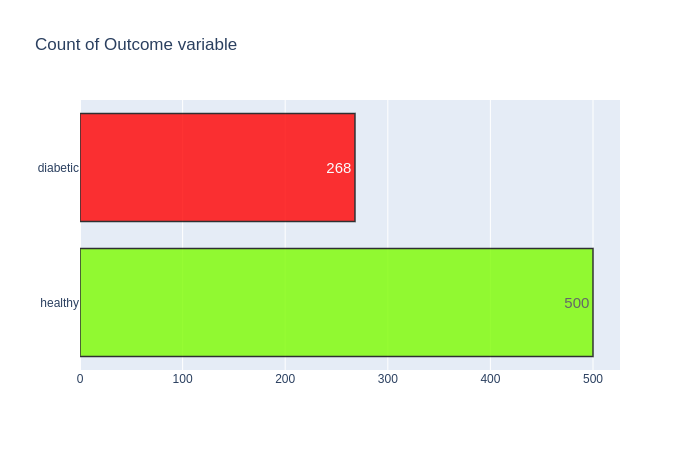
\includegraphics[width=1\textwidth]{1.png}
\caption{\label{fig:8} Diabetic v/s Healthy Subject Count obtained via target values.}
\end{figure}

\begin{figure}[ht]
\centering
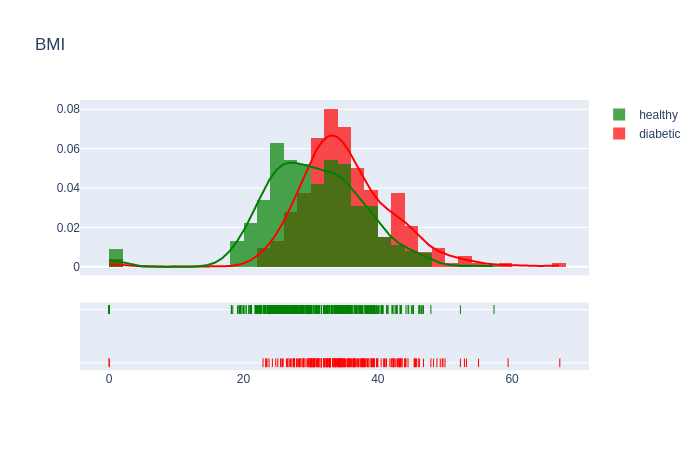
\includegraphics[width=1\textwidth]{10.png}
\caption{\label{fig:1} Subject distribution across Body Mass Index range.}
\end{figure}

\begin{figure}[ht]
\centering
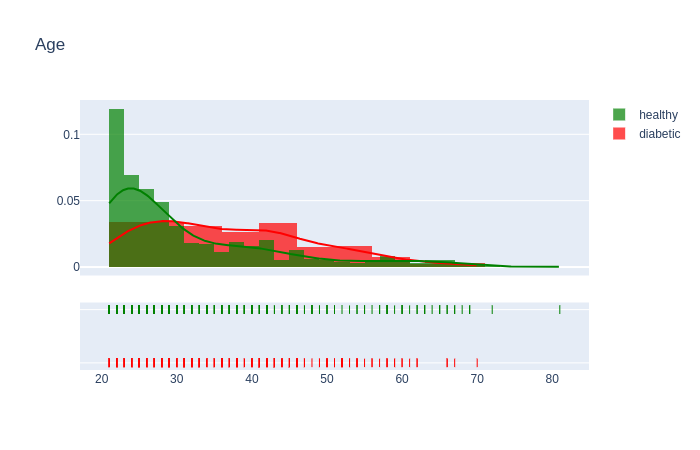
\includegraphics[width=1\textwidth]{11.png}
\caption{\label{fig:2} Subject distribution across age.}
\end{figure}

\begin{figure}[ht]
\centering
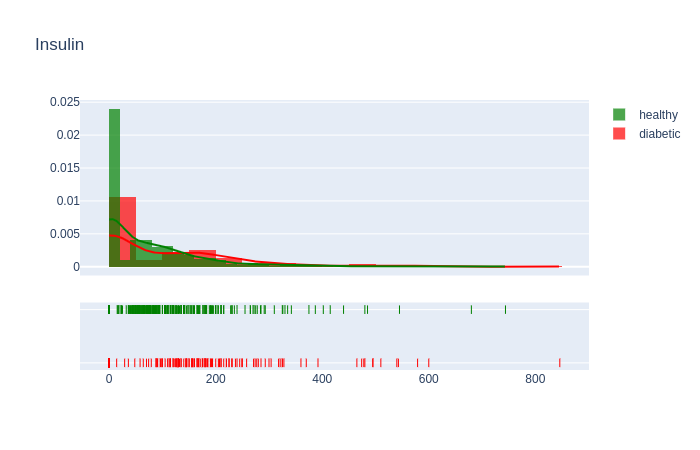
\includegraphics[width=1\textwidth]{14.png}
\caption{\label{fig:5} Subjects Insulin Distribution across ranges.}
\end{figure}

\begin{figure}[ht]
\centering
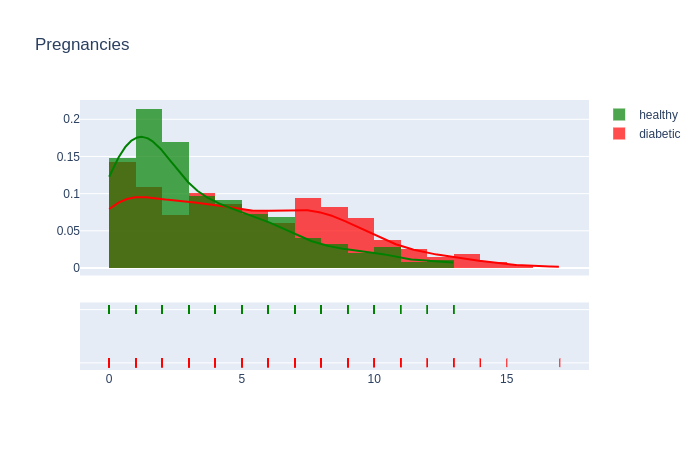
\includegraphics[width=1\textwidth]{12.png}
\caption{\label{fig:3} Subjects distribution via Pregnancies.}
\end{figure}

\begin{figure}[ht]
\centering
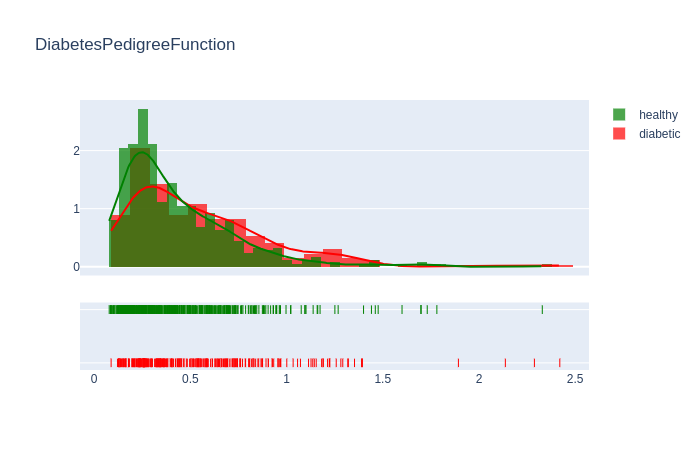
\includegraphics[width=1\textwidth]{13.png}
\caption{\label{fig:4} Subjects distribution via Diabetes Pedigree Function.}
\end{figure}


\begin{figure}[ht]
\centering
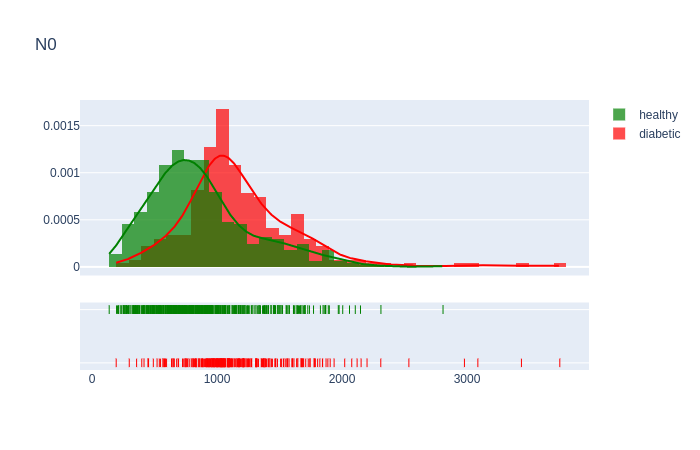
\includegraphics[width=1\textwidth]{15.png}
\caption{\label{fig:6} Plot of N0}
\end{figure}


\begin{figure}[ht]
\centering
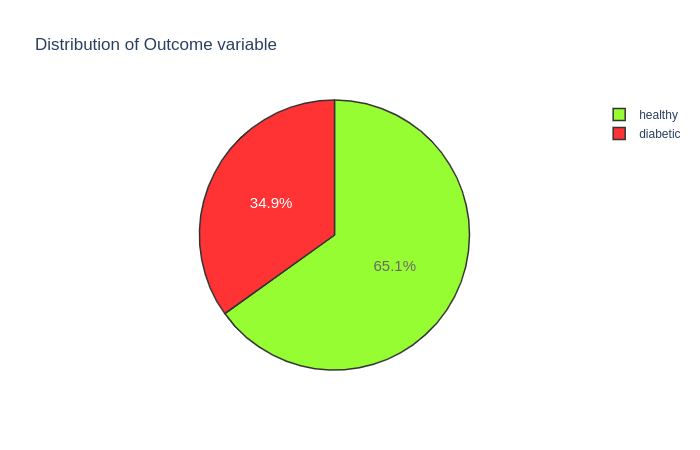
\includegraphics[width=1\textwidth]{2.png}
\caption{\label{fig:9} Diabetic v/s Healthy Subjects Percentage.}
\end{figure}

\begin{figure}[ht]
\centering
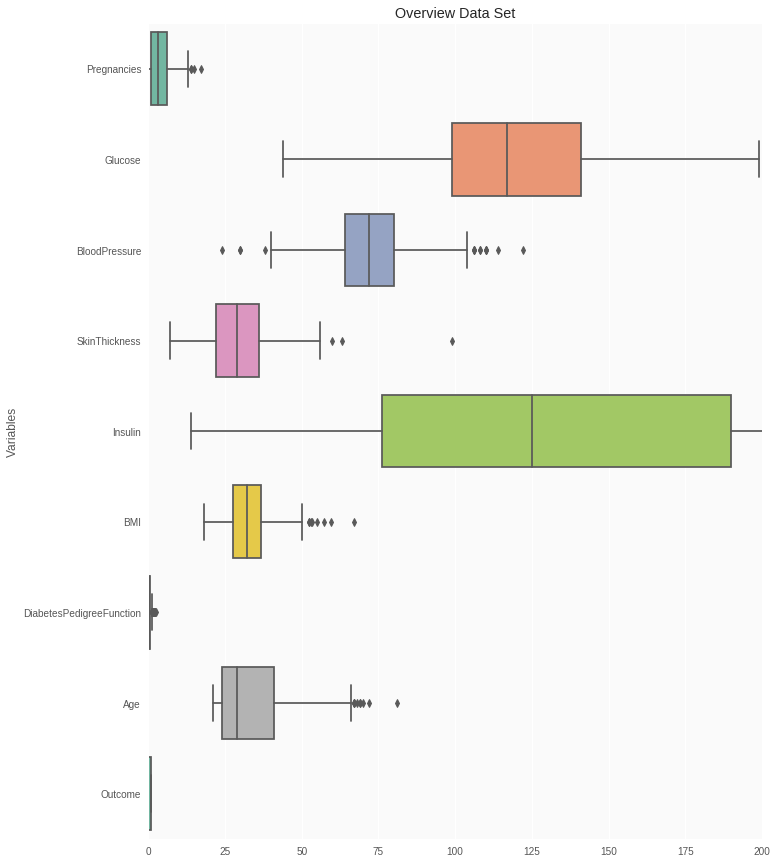
\includegraphics[width=1\textwidth]{3.png}
\caption{\label{fig:10} Boxplot for all attributes with outliers.}
\end{figure}

\begin{figure}[ht]
\centering
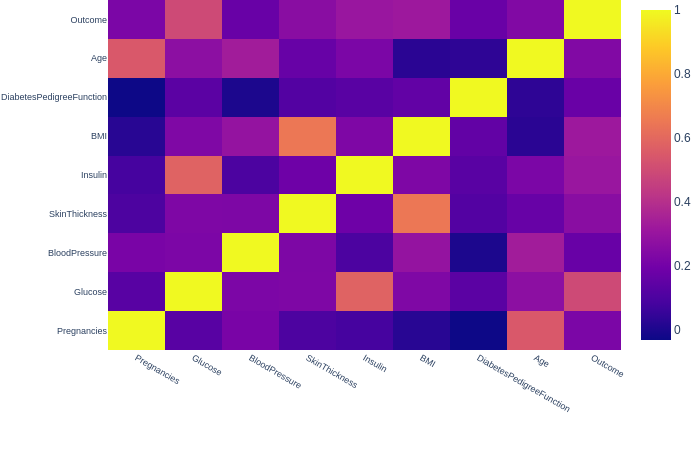
\includegraphics[width=1\textwidth]{4a.png}
\caption{\label{fig:11} Heatmap using Pearsons Correlation Coefficient.}
\end{figure}

\begin{figure}[ht]
\centering
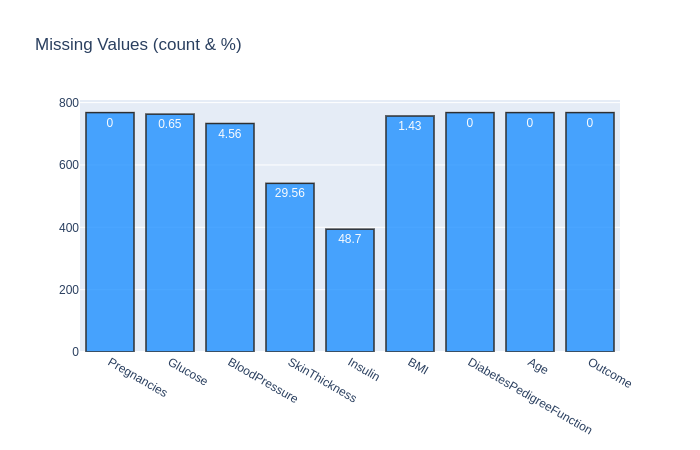
\includegraphics[width=1\textwidth]{4.png}
\caption{\label{fig:12} Number of missing values in count and percentage.}
\end{figure}

\begin{figure}[ht]
\centering
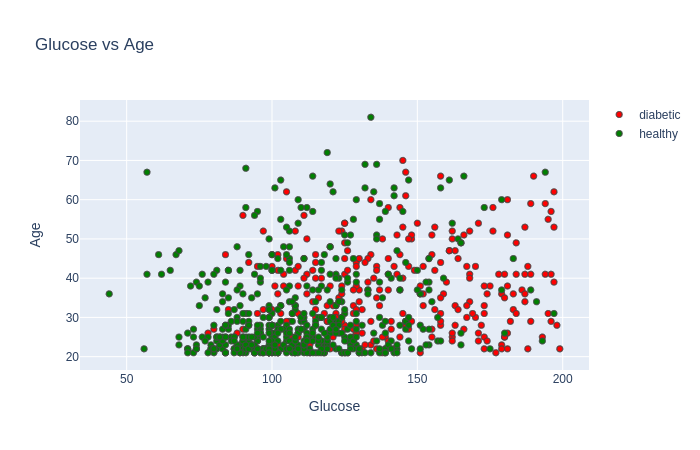
\includegraphics[width=1\textwidth]{5.png}
\caption{\label{fig:13} Glucose v/s Age scatterplot.}
\end{figure}


\begin{figure}[ht]
\centering
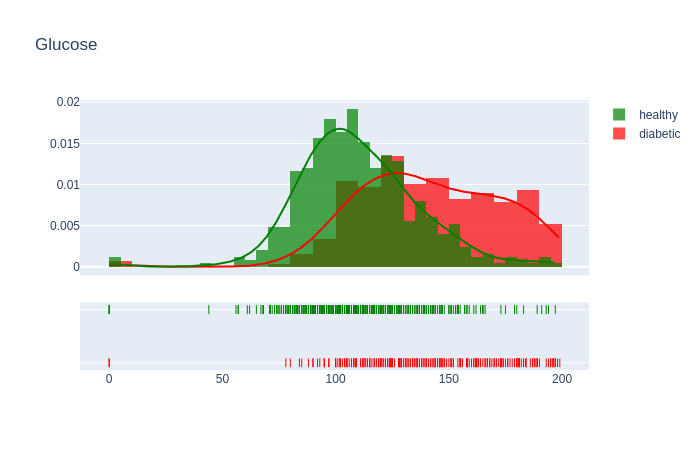
\includegraphics[width=1\textwidth]{7.png}
\caption{\label{fig:15} Subjects glucose distribution.}
\end{figure}

\begin{figure}[ht]
\centering
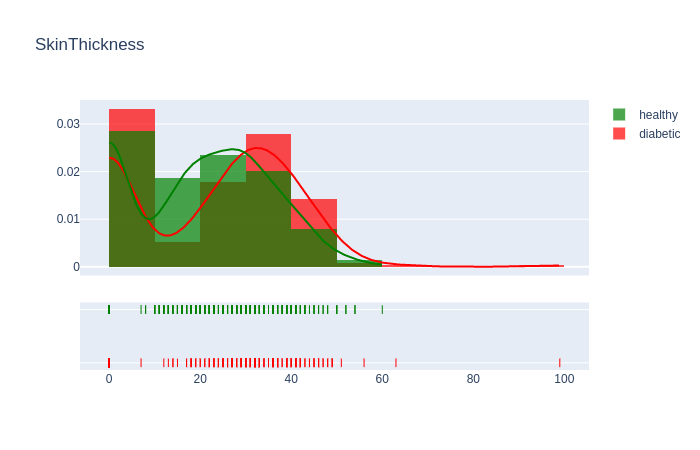
\includegraphics[width=1\textwidth]{8.png}
\caption{\label{fig:16} Skin Thickness distribution of subjects.}
\end{figure}

\begin{figure}[ht]
\centering
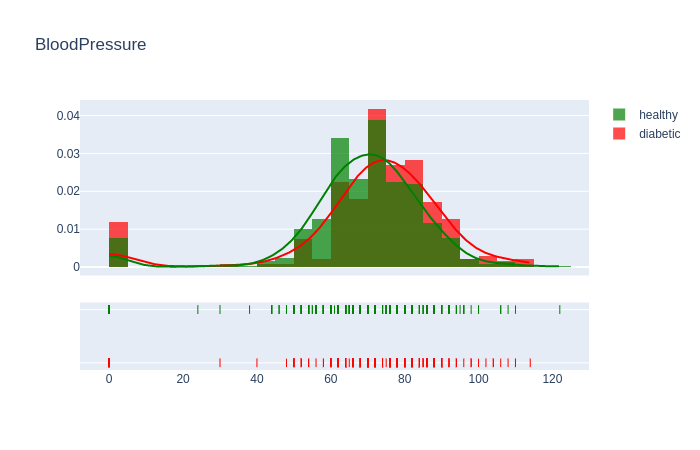
\includegraphics[width=1\textwidth]{9.png}
\caption{\label{fig:17} Blood Pressure distribution of subjects.}
\end{figure}

\begin{figure}[ht]
\centering
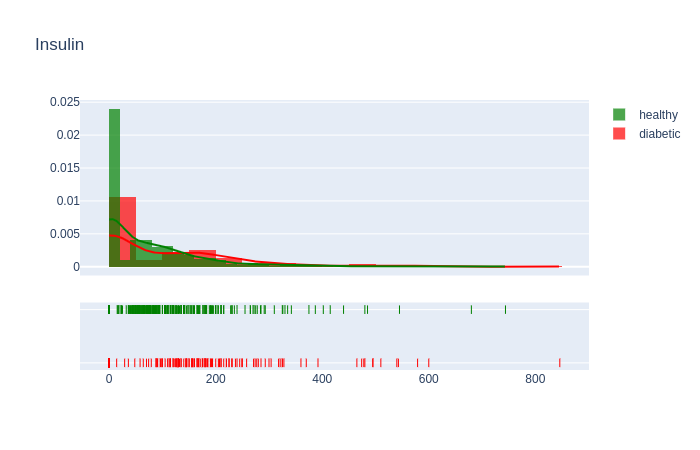
\includegraphics[width=1\textwidth]{6.png}
\caption{\label{fig:14} Subjects Insulin distributon.}
\end{figure}

\begin{figure}[ht]
\centering
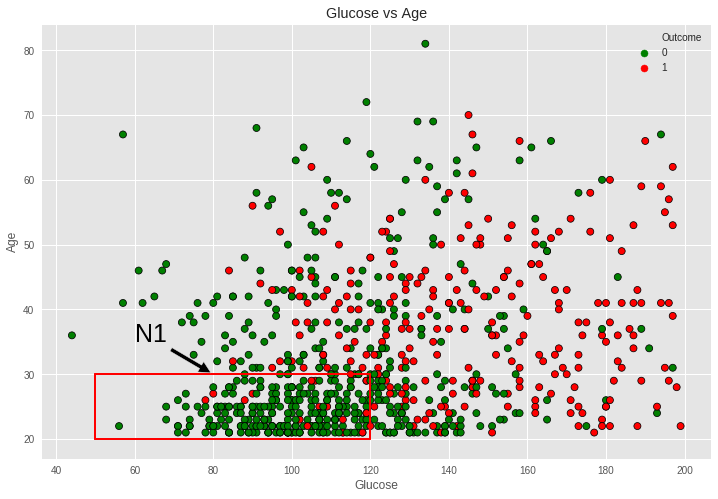
\includegraphics[width=1\textwidth]{download(1).png}
\caption{\label{fig:18} New feature N1.}
\end{figure}

\begin{figure}[ht]
\centering
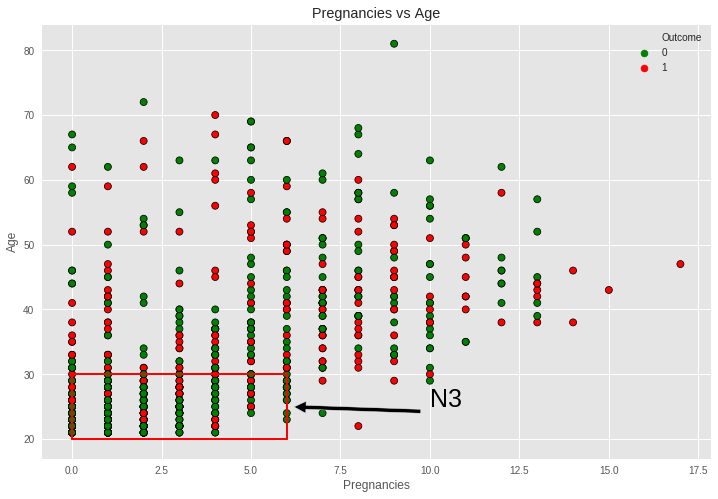
\includegraphics[width=1\textwidth]{download(2).png}
\caption{\label{fig:19} New feature N3.}
\end{figure}

\begin{figure}[ht]
\centering
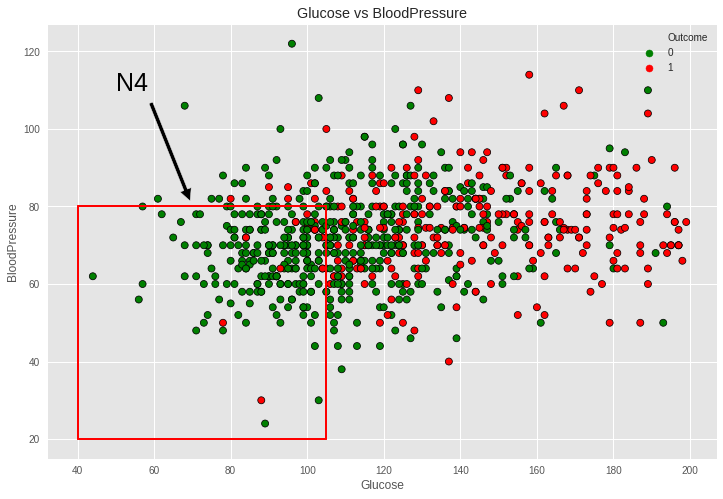
\includegraphics[width=1\textwidth]{download(3).png}
\caption{\label{fig:20}  New feature N4.}
\end{figure}

\begin{figure}[ht]
\centering
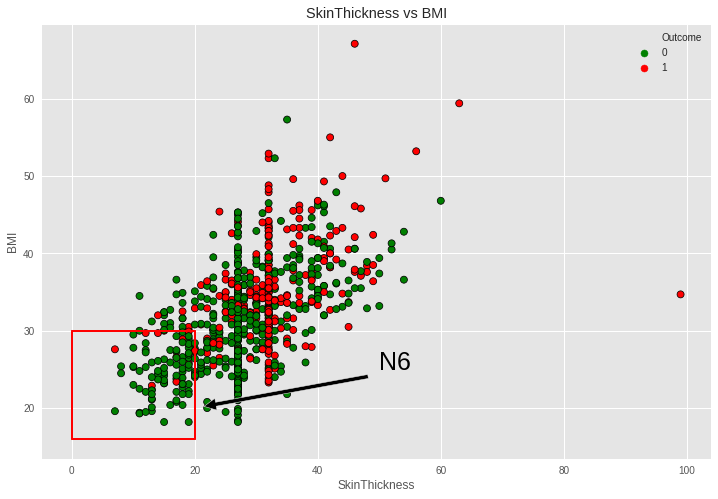
\includegraphics[width=1\textwidth]{download(4).png}
\caption{\label{fig:21}  New feature N6.}
\end{figure}

\begin{figure}[ht]
\centering
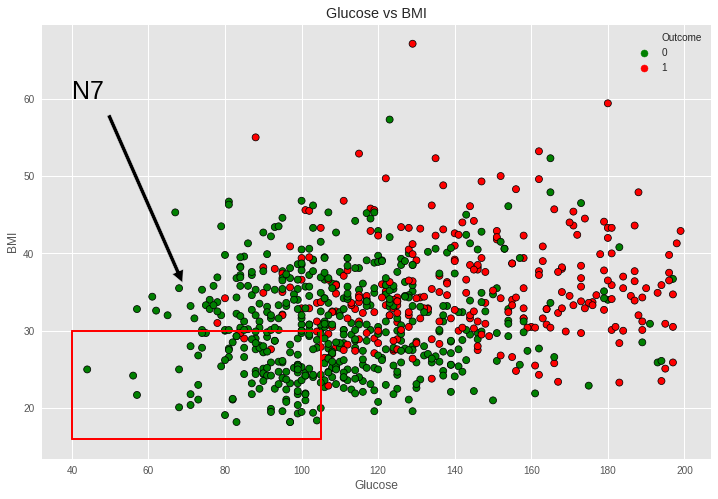
\includegraphics[width=1\textwidth]{download(5).png}
\caption{\label{fig:22}  New feature N7.}
\end{figure}

\begin{figure}[ht]
\centering
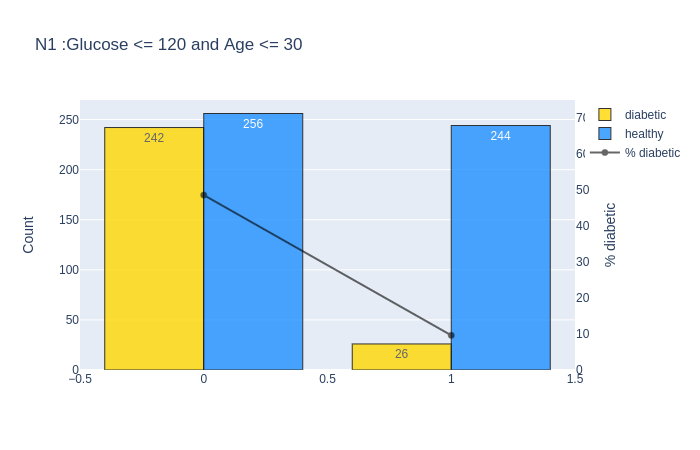
\includegraphics[width=1\textwidth]{newplot(13).png}
\caption{\label{fig:23} N1 barplot for diabetic and healthy population.}
\end{figure}

\begin{figure}[ht]
\centering
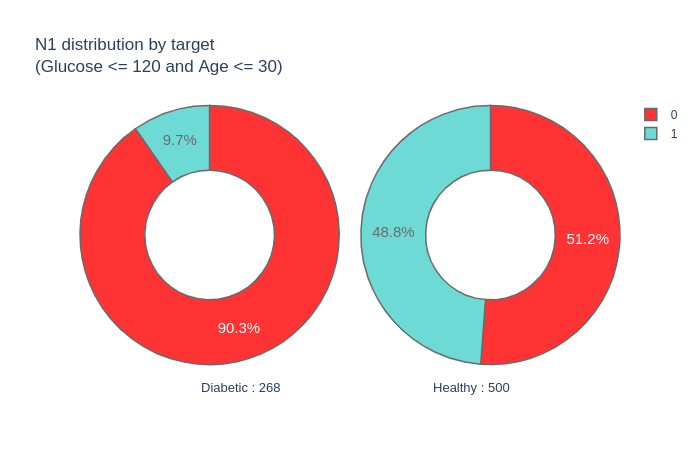
\includegraphics[width=1\textwidth]{newplot(14).png}
\caption{\label{fig:24} N1 distribution in percentage.}
\end{figure}

\begin{figure}[ht]
\centering
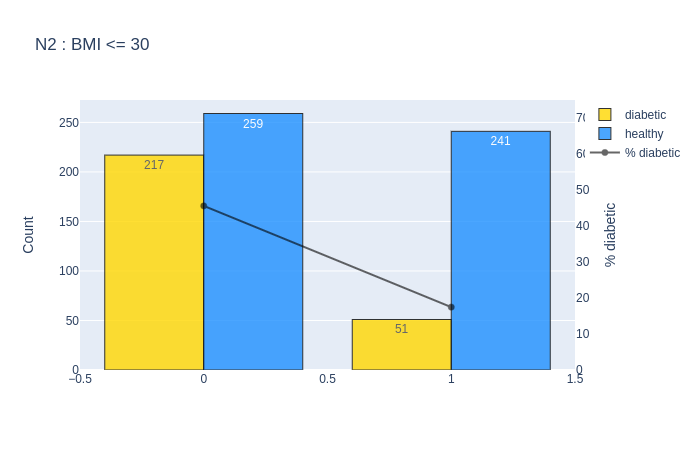
\includegraphics[width=1\textwidth]{newplot(15).png}
\caption{\label{fig:25} N2 barplot for diabetic and healthy population.}
\end{figure}

\begin{figure}[ht]
\centering
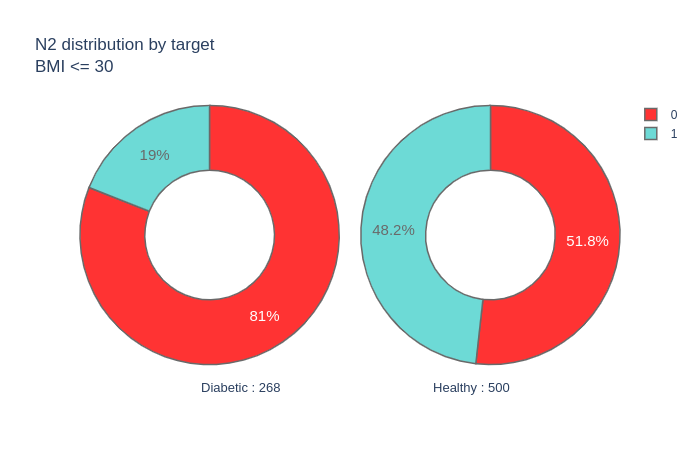
\includegraphics[width=1\textwidth]{newplot(16).png}
\caption{\label{fig:26} N2 distribution by target.}
\end{figure}

\begin{figure}[ht]
\centering
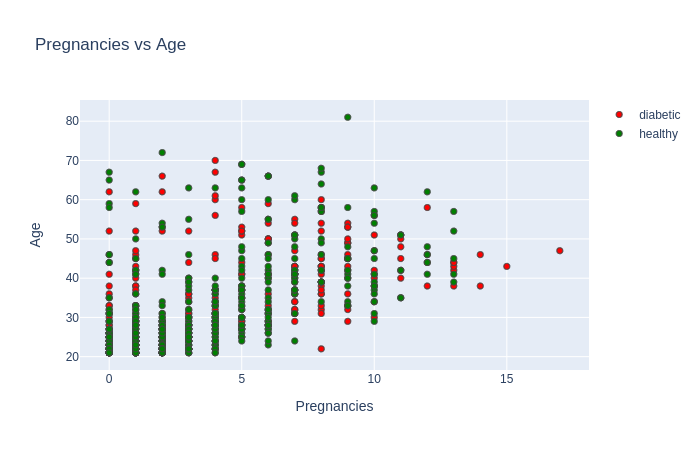
\includegraphics[width=1\textwidth]{newplot(17).png}
\caption{\label{fig:27} Pregnancies v/s age scatterplot.}
\end{figure}

\begin{figure}[ht]
\centering
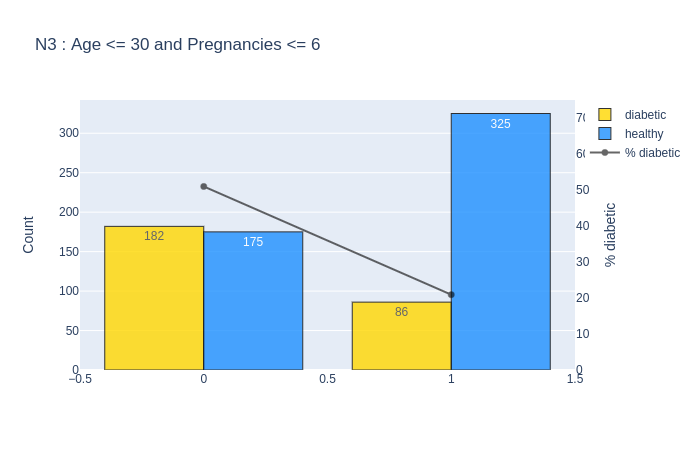
\includegraphics[width=1\textwidth]{newplot(18).png}
\caption{\label{fig:28} N3 barplot for diabetic and healthy population.}
\end{figure}

\begin{figure}[ht]
\centering
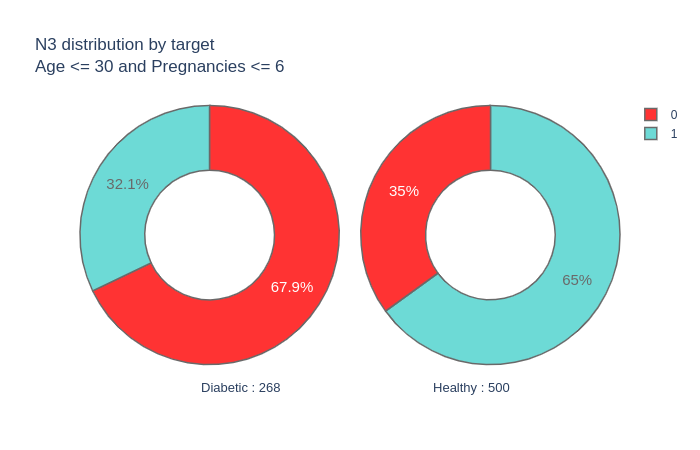
\includegraphics[width=1\textwidth]{newplot(19).png}
\caption{\label{fig:29} N3 distribution by target.}
\end{figure}

\begin{figure}[ht]
\centering
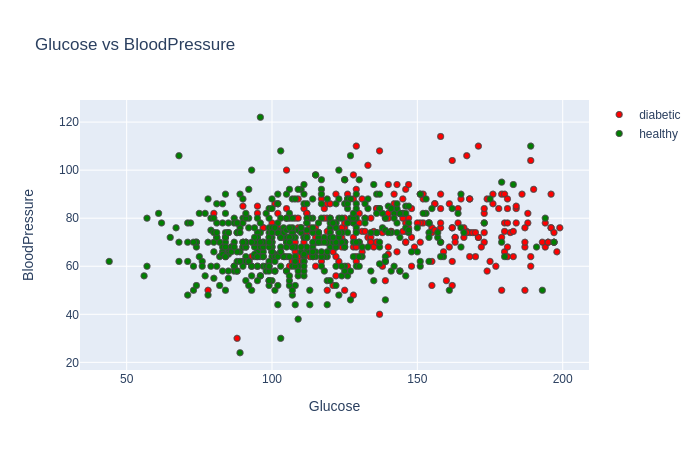
\includegraphics[width=1\textwidth]{newplot(20).png}
\caption{\label{fig:30} Glucose v/s Blood Pressure scatterplot.}
\end{figure}

\begin{figure}[ht]
\centering
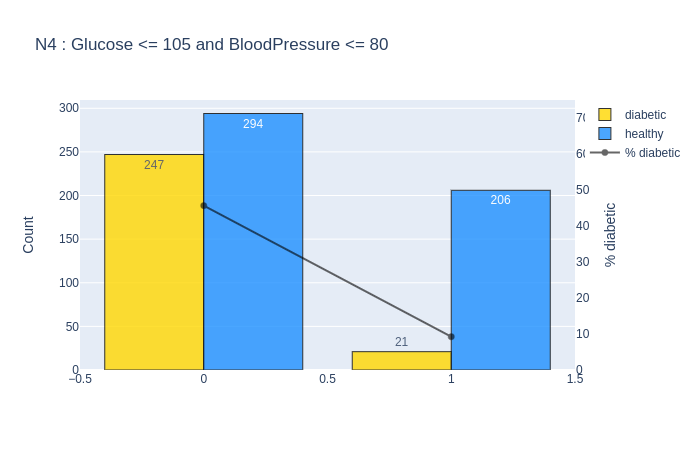
\includegraphics[width=1\textwidth]{newplot(21).png}
\caption{\label{fig:31} N4 barplot for diabetic and healthy population.}
\end{figure}

\begin{figure}[ht]
\centering
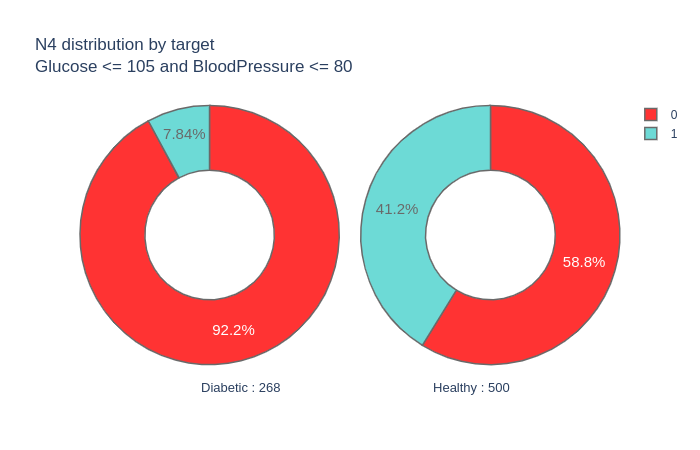
\includegraphics[width=1\textwidth]{newplot(22).png}
\caption{\label{fig:32} N4 distribution by target.}
\end{figure}

\begin{figure}[ht]
\centering
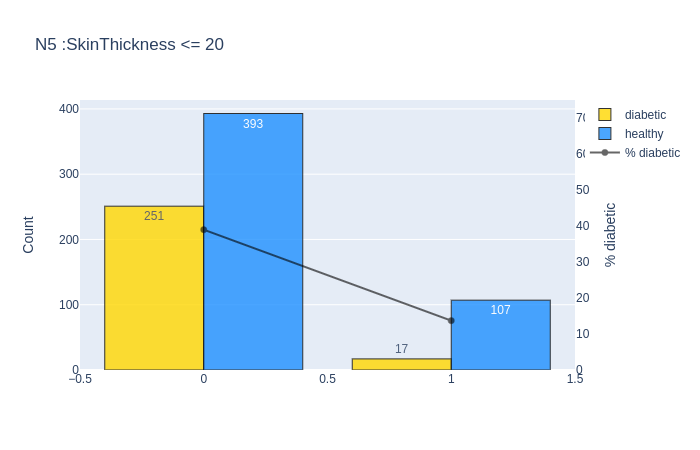
\includegraphics[width=1\textwidth]{newplot(23).png}
\caption{\label{fig:33} N5 barplot for diabetic and healthy population.}
\end{figure}

\begin{figure}[ht]
\centering
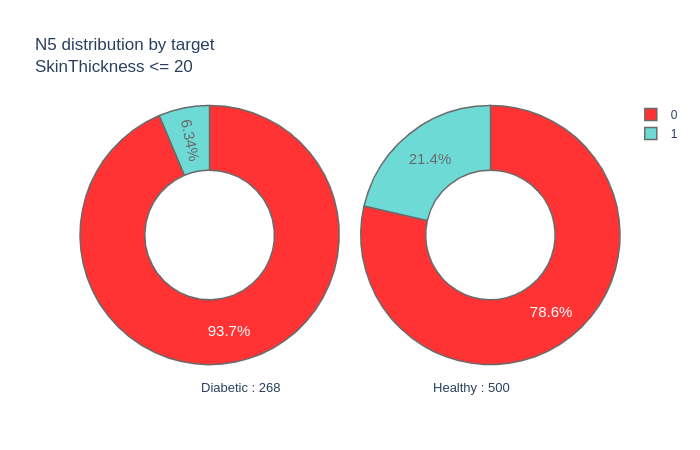
\includegraphics[width=1\textwidth]{newplot(24).png}
\caption{\label{fig:34} N5 distribution by target.}
\end{figure}

\begin{figure}[ht]
\centering
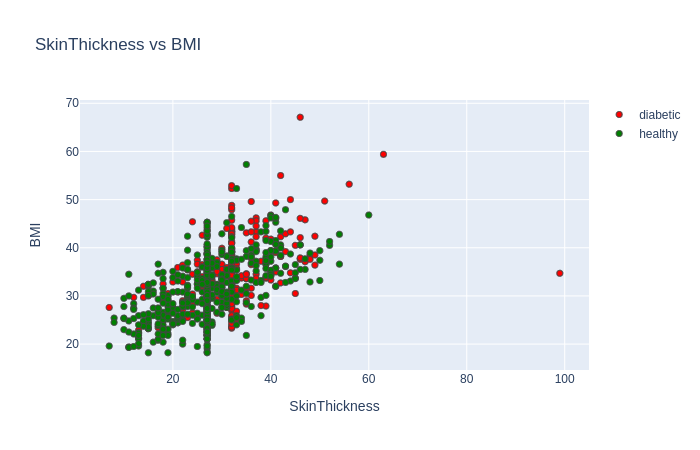
\includegraphics[width=1\textwidth]{newplot(25).png}
\caption{\label{fig:35} Skin Thickness v/s BMI scatterplot.}
\end{figure}

\begin{figure}[ht]
\centering
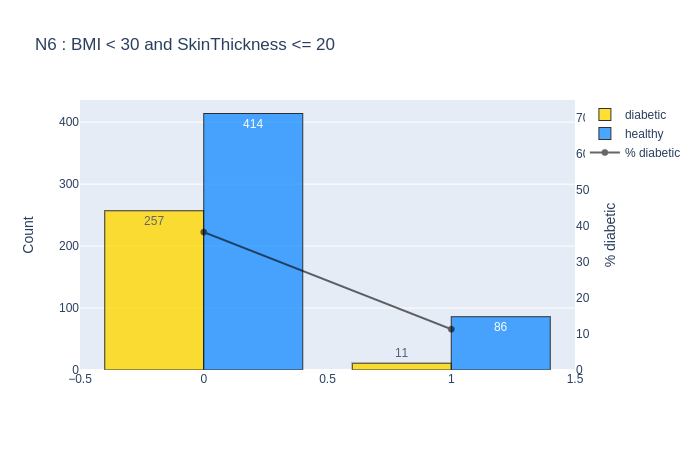
\includegraphics[width=1\textwidth]{newplot(26).png}
\caption{\label{fig:36} N6 barplot for diabetic and healthy population.}
\end{figure}

\begin{figure}[ht]
\centering
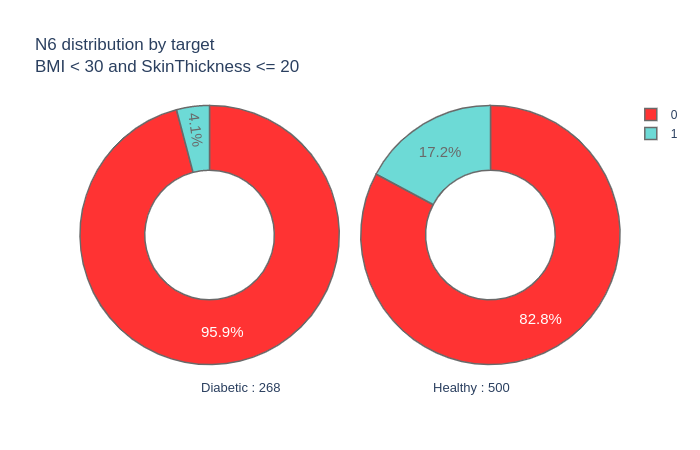
\includegraphics[width=1\textwidth]{newplot(27).png}
\caption{\label{fig:37} N6 distribution by target.}
\end{figure}

\begin{figure}[ht]
\centering
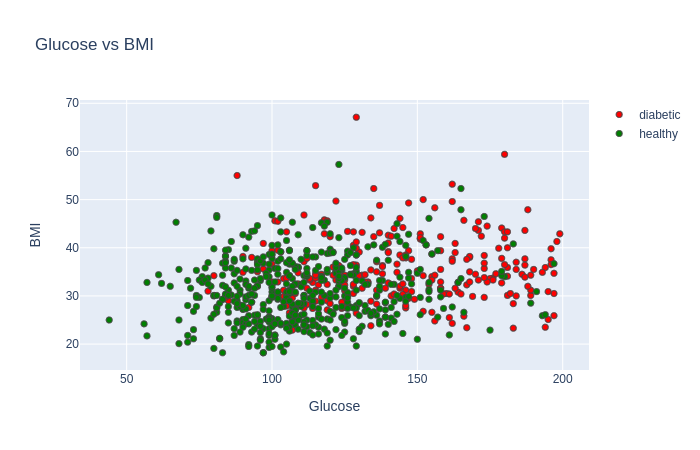
\includegraphics[width=1\textwidth]{newplot(28).png}
\caption{\label{fig:38} Glucose v/s Body Mass Index scatterplot.}
\end{figure}

\begin{figure}[ht]
\centering
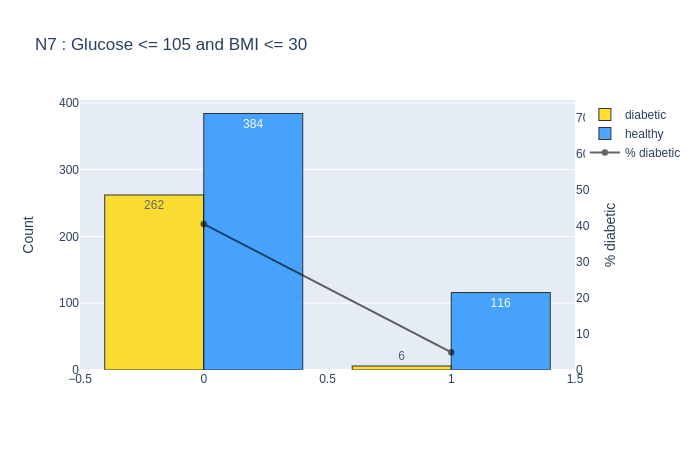
\includegraphics[width=1\textwidth]{newplot(29).png}
\caption{\label{fig:39} N7 barplot for diabetic and healthy population.}
\end{figure}

\begin{figure}[ht]
\centering
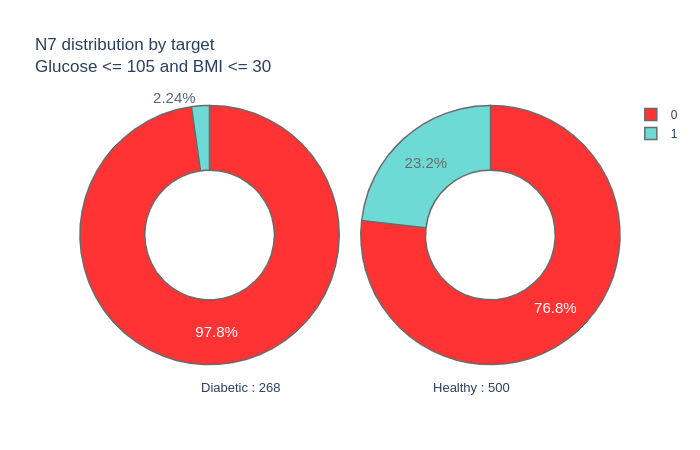
\includegraphics[width=1\textwidth]{newplot(30).png}
\caption{\label{fig:40} N7 distribution by target.}
\end{figure}

\begin{figure}[ht]
\centering
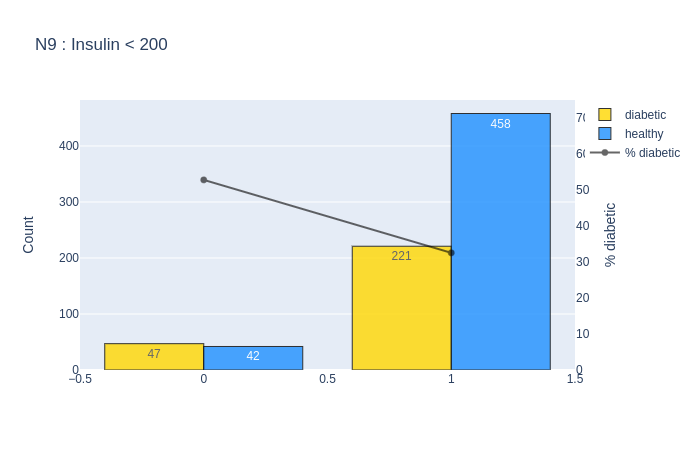
\includegraphics[width=1\textwidth]{newplot(32).png}
\caption{\label{fig:41} N9 barplot for diabetic and healthy population.}
\end{figure}

\begin{figure}[ht]
\centering
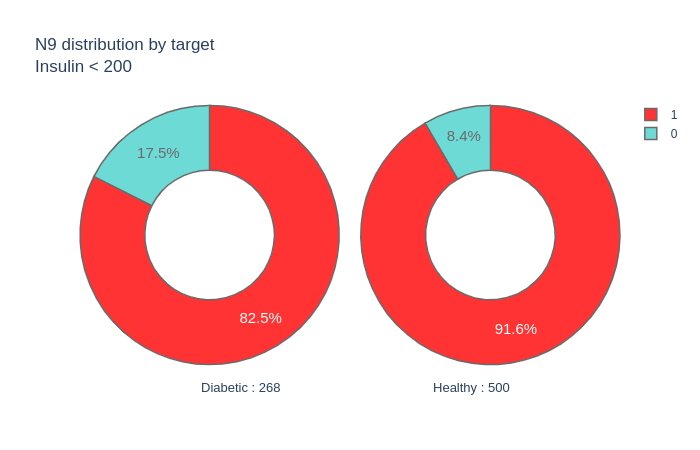
\includegraphics[width=1\textwidth]{newplot(33).png}
\caption{\label{fig:42} N9 distribution by target.}
\end{figure}

\begin{figure}[ht]
\centering
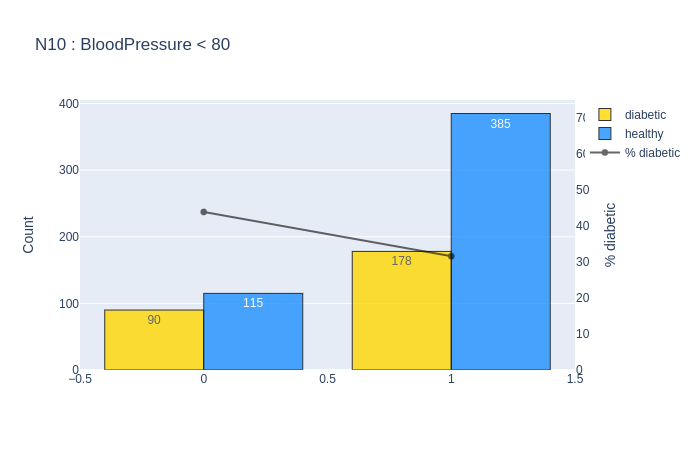
\includegraphics[width=1\textwidth]{newplot(34).png}
\caption{\label{fig:43} N10 barplot for diabetic and healthy population.}
\end{figure}

\begin{figure}[ht]
\centering
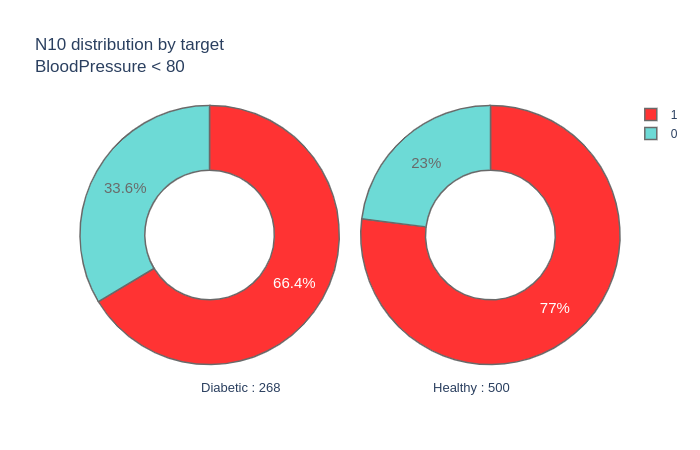
\includegraphics[width=1\textwidth]{newplot(35).png}
\caption{\label{fig:44} N10 distribution by target.}
\end{figure}

\begin{figure}[ht]
\centering
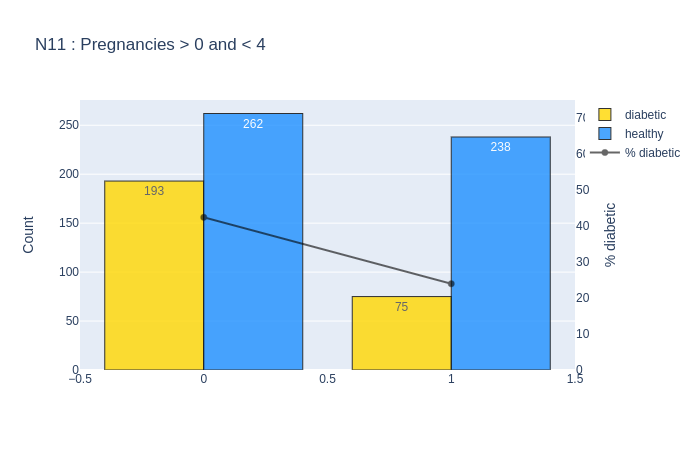
\includegraphics[width=1\textwidth]{newplot(37).png}
\caption{\label{fig:45} N11 barplot for diabetic and healthy population.}
\end{figure}

\begin{figure}[ht]
\centering
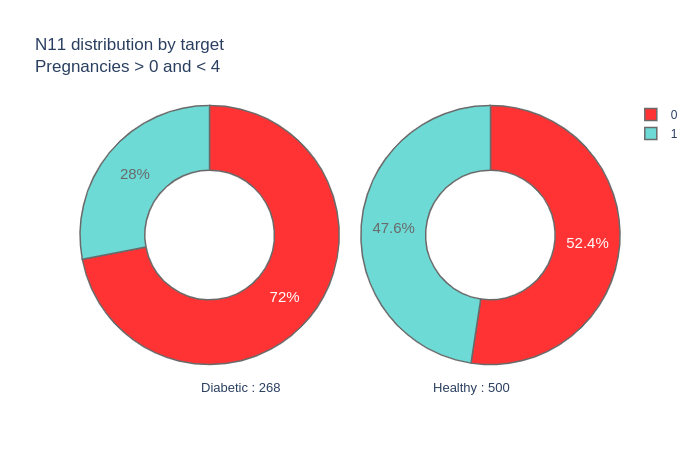
\includegraphics[width=1\textwidth]{newplot(38).png}
\caption{\label{fig:46} N11 distribution by target.}
\end{figure}

\begin{figure}[ht]
\centering
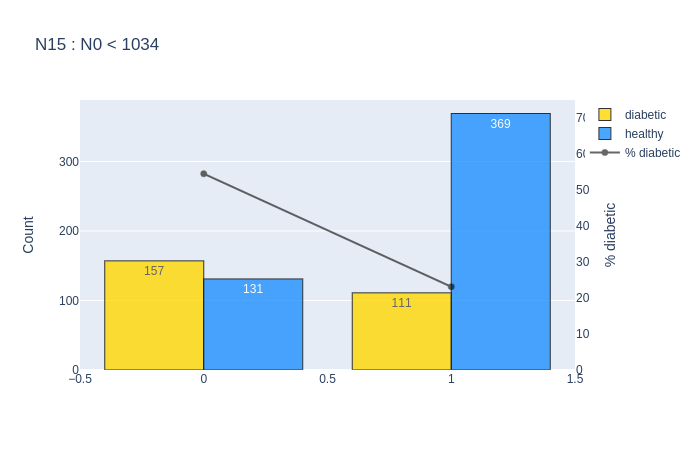
\includegraphics[width=1\textwidth]{newplot(40).png}
\caption{\label{fig:47} N15 barplot for diabetic and healthy population.}
\end{figure}

\begin{figure}[ht]
\centering
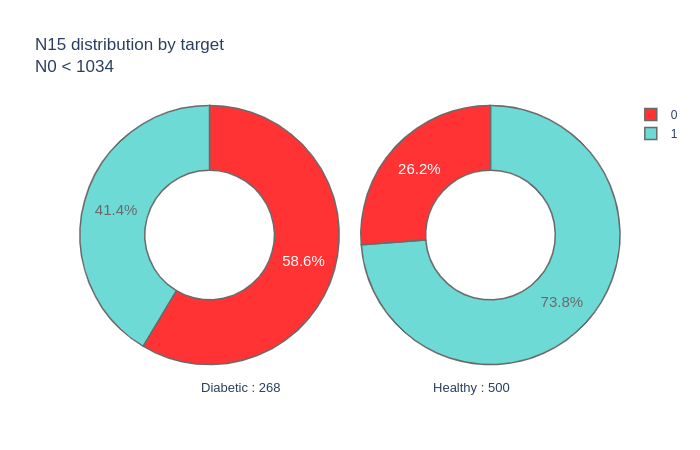
\includegraphics[width=1\textwidth]{newplot(41).png}
\caption{\label{fig:48} N15 distribution by target.}
\end{figure}

\clearpage
\newpage

\section{Web and API Interface Images}
\vspace{3cm}
\begin{figure}[ht]
\centering
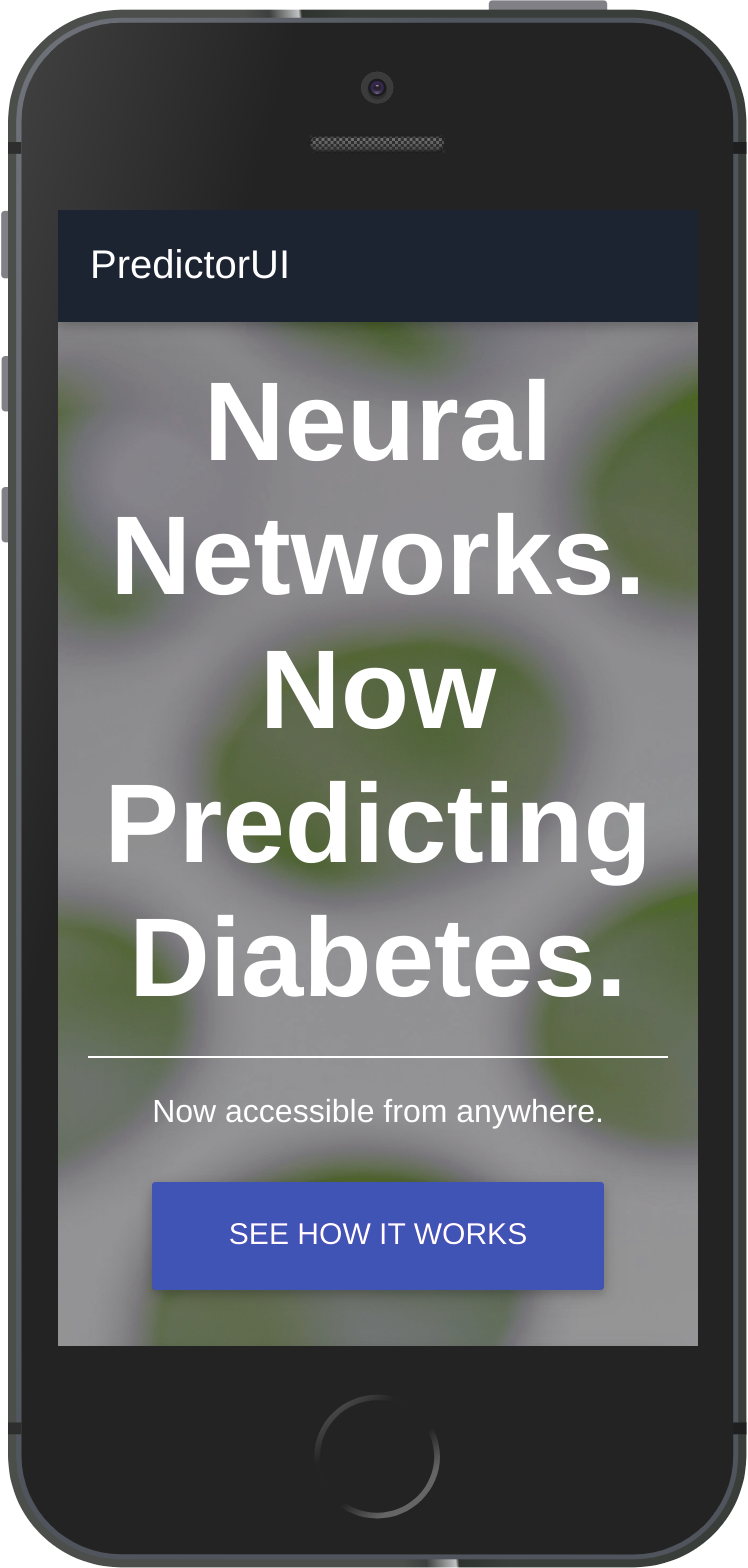
\includegraphics[width=0.45\textwidth]{1se.png}
\caption{\label{fig:50} Landing Page for website user interface depicted on iPhone 5SE.}
\end{figure}
\begin{figure}[ht]
\centering
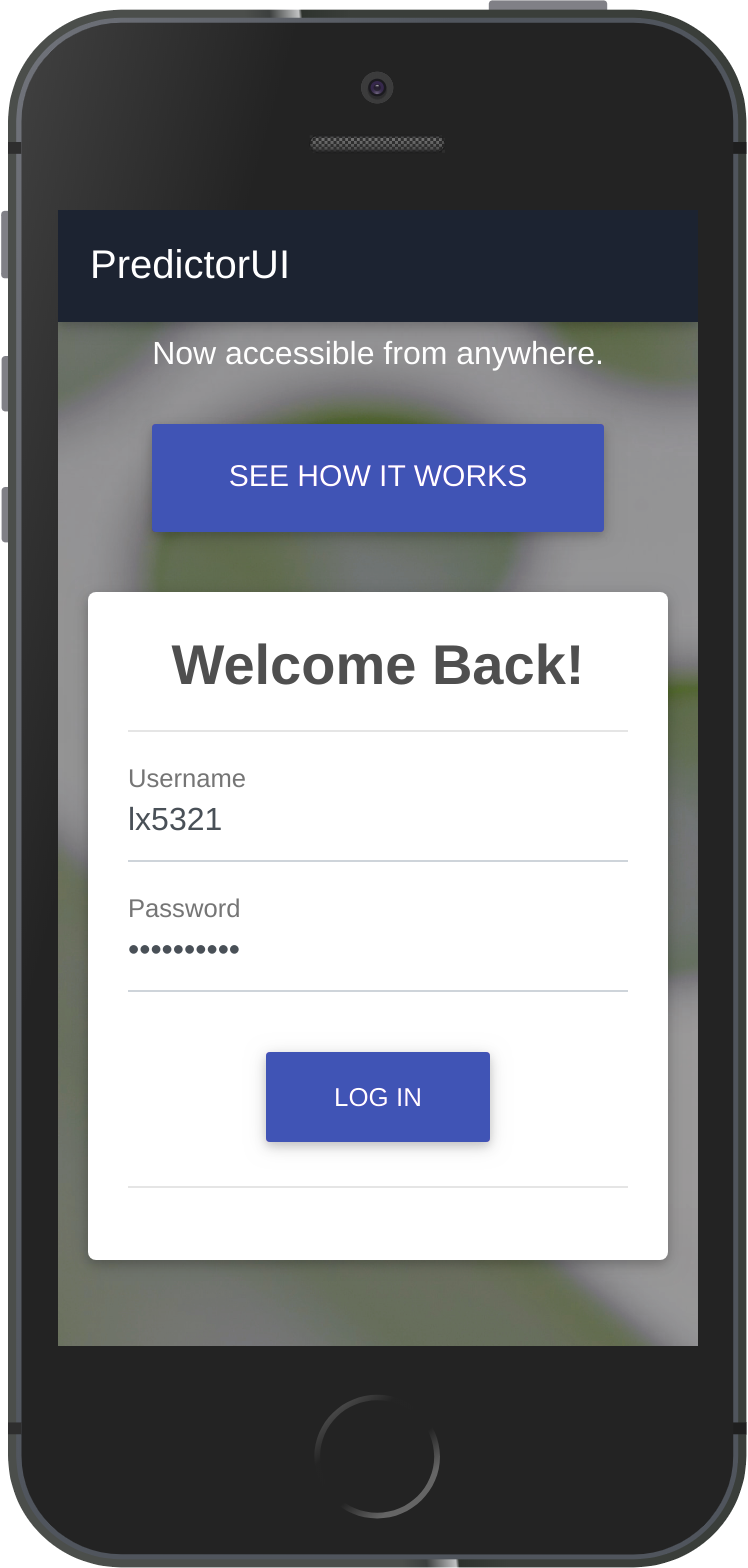
\includegraphics[width=0.3\textwidth]{2se.png}
\caption{\label{fig:51} User Login Page for website user interface depicted on iPhone 5SE.}
\end{figure}
\begin{figure}[ht]
\centering
\includegraphics[width=0.3\textwidth]{3se.png}
\caption{\label{fig:52} Interactive and responsive graphs with touch or mouse hover capable interaction depicted on iPhone 5SE.}
\end{figure}
\begin{figure}[ht]
\centering
\includegraphics[width=0.3\textwidth]{4se.png}
\caption{\label{fig:53} Percentage of predicted risk for every patient.}
\end{figure}
\begin{figure}[ht]
\centering
\includegraphics[width=0.3\textwidth]{5se.png}
\caption{\label{fig:54} Modal based interaction for specific activities.}
\end{figure}
\begin{figure}[ht]
\centering
\includegraphics[width=0.3\textwidth]{6se.png}
\caption{\label{fig:55} User interface for doctors. Kept to a minimal for hassle free operation.}
\end{figure}
\begin{figure}[ht]
\centering
\includegraphics[width=0.3\textwidth]{7se.png}
\caption{\label{fig:56} AJAX enable live search for patients.}
\end{figure}
\begin{figure}[ht]
\centering
\includegraphics[width=0.45\textwidth]{8se.png}
\caption{\label{fig:57} Form Validation and error handling to prevent erroneous values in database.}
\end{figure}

{
\clearpage
\begin{landscape}
\begin{figure}[ht]
\centering
\includegraphics[width=1.5\textwidth]{nodejsapi.png}
\caption{\label{fig:58} API built with Node.js capable of interfacing w/ database.}
\end{figure}
\end{landscape}
}
\clearpage
\newpage
\nocite{*}
\bibliography{bib} 
\bibliographystyle{plain}
\end{document}
